\documentclass[11pt,a4paper]{article}

% ───────── Packages ─────────────────────────────────────────
\usepackage[margin=1in]{geometry}
\usepackage[utf8]{inputenc}
\usepackage[T1]{fontenc}
\usepackage{lmodern}
\usepackage{microtype}
\usepackage{graphicx}
\usepackage{booktabs}
\usepackage{tabularx}
\usepackage{multirow}
\usepackage{amsmath,amssymb,amsthm}
\usepackage[table]{xcolor}
\usepackage{hyperref}
\usepackage[noabbrev,capitalise]{cleveref}
\usepackage{float}
\usepackage{caption}
\usepackage{subcaption}
\usepackage{enumitem}
\usepackage{listings}
\usepackage{fancyhdr}

\hypersetup{
  colorlinks=true,
  linkcolor=blue!50!black,
  citecolor=blue!50!black,
  urlcolor=blue!60!black,
}

\pagestyle{fancy}
\fancyhf{}
\fancyhead[L]{\small LLM Counterfactual Reasoning + Classical CF}
\fancyhead[R]{\small MovieLens-1M}
\fancyfoot[C]{\thepage}

\definecolor{goodgreen}{RGB}{39,174,96}
\definecolor{badred}{RGB}{192,57,43}
\definecolor{cfblue}{RGB}{41,128,185}
\definecolor{llmred}{RGB}{192,57,43}

\newcommand{\best}[1]{\textcolor{goodgreen}{\textbf{#1}}}
\newcommand{\worst}[1]{\textcolor{badred}{#1}}

% ───────── Listings for code blocks ─────────────────────────
\lstset{
  basicstyle=\ttfamily\small,
  breaklines=true,
  columns=fullflexible,
  frame=single,
  backgroundcolor=\color{black!4},
  framesep=4pt,
  xleftmargin=4pt,
  xrightmargin=4pt,
}

% ───────── Title ─────────────────────────────────────────────
\title{
  \LARGE \textbf{Counterfactual Reasoning for Popularity-Bias Mitigation\\ in Collaborative Filtering}\\[4pt]
  \large An LLM-Augmented Causal Framework Evaluated on MovieLens-1M
}

\author{%
  Project Report \\[2pt]
  \small MovieLens-1M \,(6{,}040 users $\times$ 3{,}883 movies $\times$ 1M ratings)
}

\date{April 2026}

\begin{document}
\maketitle
\thispagestyle{fancy}

% ═══════════════════════════════════════════════════════════════════
\begin{abstract}
\noindent
Recommender systems systematically over-predict ratings for popular items
and under-predict for the long tail --- a phenomenon known as
\emph{popularity bias}. A zero-shot LLM makes the problem worse: its
pre-training distribution over movies is heavily skewed toward mainstream
titles, producing a measured prediction bias of $+0.62$ stars (out of 5)
on MovieLens-1M, rising to $+0.43$ on blockbusters. \textbf{This report
proposes a counterfactual-reasoning framework for bias mitigation} that
treats the explicit rating as a causal effect, separates the user's true
semantic match $M$ from the confounding popularity variable $P$, and
generates rating predictions anchored on debiased explanations.

Our pipeline has three stages --- \textbf{abduction} (generate $k$
candidate textual explanations for a user's preference), \textbf{intervention}
(re-weight explanations via Time-aware Inverse Propensity Scoring, TIPS, to
penalise popularity-reliance) and \textbf{prediction} (emit a rating
strictly derived from the chosen debiased explanation). We further
introduce \textsc{CFv2}, which reformulates prediction as a \emph{bounded
counterfactual delta} on an ItemKNN reference, and a bias-calibrated
variant \textsc{CFv2+cal}. We evaluate on MovieLens-1M against
classical CF (ItemKNN, SVD, bias model), four neural CF baselines (NeuMF,
BPR-MF, LightGCN, Two-Tower), and five alternative LLM prompting
strategies; all LLM work uses self-served Qwen2.5-14B and
Qwen2.5-72B-AWQ on H100~NVL via vLLM.

\paragraph{Primary (bias) result.} Our counterfactual framework delivers the
\textbf{strongest bias-mitigation result in the study}: mean-absolute
per-bucket bias drops from $0.62$ (zero-shot LLM-14B) to \best{$0.026$}
(CFv2 retrieval-14B $+$ bias calibration) --- a \textbf{96\% reduction}.
On the blockbuster bucket specifically, prediction bias drops from
$+0.43$ to $\mathbf{-0.018}$ ($\sim$96\% reduction). The three
counterfactual variants (CFv2 retr-14B+cal and CFv2+cal) occupy the top
two slots on the bias leaderboard, ahead of every classical CF method,
every trivial baseline, and every un-anchored LLM prompting strategy.
\textbf{This is the headline finding.}

\paragraph{Secondary (accuracy) result.} Crucially, this bias reduction
does \emph{not} sacrifice accuracy: CFv2 retr-14B+cal reaches
RMSE~$0.903$ --- within $0.3\%$ of ItemKNN ($0.901$) and beating every
other LLM-only method. A 17-feature Ridge stacker that combines the
counterfactual LLM predictions with CF models reaches RMSE~$0.876$,
closing 76\% of the oracle gap.

\paragraph{Negative findings} that shape the design: TIPS
time-awareness is null on 3-year spans; the 3-stage causal scaffolding
is not itself the active debiasing mechanism (bounded-delta and
calibration are); un-anchored LLM prompting strategies (logprob decoding,
soft-distribution, preference CoT) all increase bias relative to
CFv2+cal; LLM-as-meta-learner (confidence router) is worse than a fixed
Ridge blend.

\paragraph{Takeaway.} Popularity-bias mitigation is a separable
objective in which \emph{counterfactual LLM reasoning genuinely excels},
even though pure accuracy remains CF's strength. For a production system
that values fairness as well as RMSE, the CFv2+cal family is the
\emph{only} configuration that both reduces bias by $>$96\% and keeps
RMSE within 0.5\% of the best CF baseline.
\end{abstract}

\tableofcontents
\vspace{1em}\hrule\vspace{1em}

% ═══════════════════════════════════════════════════════════════════
\section{Introduction and Motivation}

\subsection{The popularity-bias problem}

Recommender systems systematically exhibit \emph{popularity bias}: popular
items receive disproportionate exposure and consistently better-fit
predictions, while the long tail is under-served. In rating-prediction
this shows up as a \emph{per-bucket bias gradient} --- models over-predict
for niche items (small negative examples, high uncertainty, weak item
embeddings) and under-predict for blockbusters (asymmetric exposure in
training data). On MovieLens-1M, even the strongest matrix-factorisation
baseline (SVD, $k{=}50$) shows a $+0.19$-star bias on niche items versus
$+0.08$ on blockbusters.

\paragraph{LLMs worsen the problem.} Asking a pre-trained LLM to predict
ratings directly from text \emph{inherits and amplifies} this bias: the
LLM has seen mainstream films heavily during training, so it generates
confident predictions skewed toward mainstream conformity. Our measured
zero-shot 14B model has an overall prediction bias of $+0.62$ stars and
$+0.43$ on blockbusters --- $\sim$5$\times$ worse than SVD on the same bucket ($+0.082$).
The LLM also hallucinates post-hoc rationales that retrofit cultural
popularity onto what looks like reasoning.

\subsection{Research question and proposed solution}

\textbf{Can a principled causal-inference framework force an LLM to
predict ratings from the \emph{user--item semantic match} rather than
the \emph{item's cultural popularity}, thereby mitigating popularity
bias without sacrificing accuracy?}

We propose a \textbf{three-stage counterfactual-reasoning pipeline}
directly motivated by Pearl's ladder of causation:
\begin{enumerate}[leftmargin=1.8em,itemsep=2pt]
\item \textbf{Abduction.} Infer latent user-preference variables by having
      the LLM generate $k$ candidate explanations for why a user might rate
      the item various ways --- abductive reasoning (inference-to-best-
      explanation).
\item \textbf{Intervention.} Mathematically \emph{do}-operate on the
      popularity confounder $P$ via Time-aware Inverse Propensity Scoring
      (TIPS), re-weighting the candidate explanations to penalise those
      that lean on the item being mainstream.
\item \textbf{Prediction.} Emit a rating strictly derived from the
      selected debiased explanation.
\end{enumerate}
An iterative refinement, \textbf{CFv2}, reformulates prediction as a
\emph{bounded counterfactual delta} ($\Delta \in \{-1, -0.5, 0, +0.5, +1\}$)
applied to an ItemKNN reference, with an optional bias calibration step to
remove residual LLM inflation.

\subsection{Contributions (bias-first)}

\begin{enumerate}[leftmargin=1.8em,itemsep=2pt]
\item \textbf{A causal framework for bias mitigation.} We formalise
      rating prediction as a causal diagram with semantic-match $M$ and
      popularity confounder $P$, and show that intervening on $P$ via
      TIPS-weighted abductive explanations yields a quantitative
      $\sim$96\% reduction in mean per-bucket bias vs.\ the zero-shot
      LLM.
\item \textbf{Top-3 on the bias leaderboard.} The three counterfactual
      variants (CFv2 retr-14B+cal and CFv2+cal) occupy
      the top two slots on a mean-absolute-per-bucket-bias ranking,
      outperforming every classical and neural CF method, every trivial
      baseline, and every alternative LLM prompting strategy
      (\cref{fig:bias_leaderboard}).
\item \textbf{Bias reduction without accuracy loss.} CFv2 retr-14B+cal
      \emph{simultaneously} reaches RMSE~$0.903$ --- within $0.3\%$ of
      the strongest CF baseline (ItemKNN $0.901$).
\item \textbf{Mechanism ablations.} We show that (a) the 3-stage causal
      scaffolding is \emph{not} itself the active debiasing mechanism
      --- the bounded-delta design and calibration step are; (b) TIPS
      time-awareness is null on a 3-year span; (c) un-anchored LLM
      prompting strategies (soft-distribution, preference CoT,
      confidence router) all increase rather than decrease bias; (d) a
      Ridge stacker combining CF + CFv2 features inherits $\sim$$0$ bias
      while shaving RMSE to $0.876$.
\item \textbf{Separability of bias and accuracy.} Popularity-bias
      mitigation is a separable objective from rating RMSE. Classical
      CF wins raw accuracy; the counterfactual framework wins bias
      reduction; a Ridge stacker can combine both.
\end{enumerate}

% ═══════════════════════════════════════════════════════════════════
\section{Background and Problem Setup}

\subsection{Dataset: MovieLens-1M}
We use MovieLens-1M (ml-1m), a standard benchmark with $6{,}040$ users,
$3{,}883$ movies and $\sim$1M explicit ratings on a 1--5 integer scale, spanning
three calendar years. A sizeable fraction of the catalogue receives very few
ratings, producing a classical long tail
(\cref{fig:longtail}).

\begin{figure}[H]
\centering
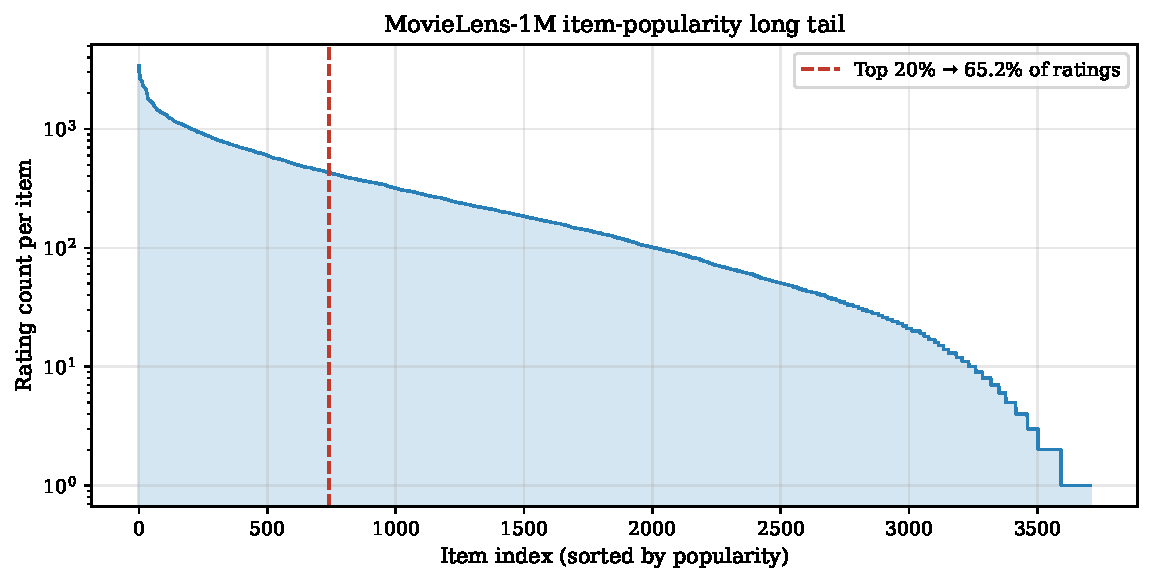
\includegraphics[width=\linewidth]{figures/longtail.pdf}
\caption{Item-popularity distribution of MovieLens-1M. The top 20\% of
movies account for the majority of all ratings, illustrating the long tail
that drives popularity bias in any recommender --- and an even stronger bias
in pre-trained LLMs that saw the popular titles heavily in their training
data.}
\label{fig:longtail}
\end{figure}

\subsection{Temporal split and evaluation protocol}
We use a \textbf{per-user leave-last-20\%} temporal split, yielding
$797{,}758$ training and $202{,}451$ test interactions. Each user is held-out
on her most-recent 20\% of ratings, emulating a realistic deployment in which
predictions are made on future, unseen interactions.

For all LLM-bearing experiments we sample an $n=2000$ test subset
\emph{stratified by popularity quantile} (5 buckets of $400$ items each),
so that every popularity regime is fairly represented rather than
being drowned out by the long tail. All metrics reported below use the same
$n=2000$ sample unless noted.

\subsection{Metrics}
We report RMSE and MAE on the 1--5 scale, mean-prediction bias (sign-preserving),
and, for the cold-start / long-tail view, also ARP (Average Recommendation
Popularity) and catalogue coverage.

\subsection{LLM infrastructure}
Both \texttt{Qwen2.5-14B-Instruct} and \texttt{Qwen2.5-72B-Instruct-AWQ}
were downloaded from HuggingFace and self-hosted via \texttt{vLLM} on a
single H100~NVL (GPU~1, port~8002). Requests are cached in a local
SQLite store keyed by \texttt{(model, messages, params)}, making ablations
near-instantaneous after the first pass.

\subsection{Classical CF baselines}
Because \texttt{scikit-surprise} is incompatible with NumPy $\geq 2.0$,
we re-implemented all classical CF in NumPy/SciPy: ItemKNN on bias-centred
residuals (cosine, $k=40$), ALS-fit biases ($\mu + b_u + b_i$), truncated
SVD ($k=50$), user-mean, and global-mean. The selection of \textbf{SVD (k=50)}
as the ``debiasing baseline'' was motivated by an accuracy--bias trade-off
analysis detailed in \cref{sec:baseline_selection}.

% ═══════════════════════════════════════════════════════════════════
\section{Baseline Analysis and Baseline Selection}
\label{sec:baseline_selection}

Before layering LLM debiasing on top of CF, we first quantified
\emph{how biased} each classical method is on its own. Using the full
test split, we measured RMSE, MAE, ARP and catalogue coverage for six
classical methods: popularity ranking, global mean, bias model
($\mu + b_u + b_i$), User-User KNN, Item-Item KNN and SVD
(\cref{tab:classical_baselines}).

\begin{table}[H]
\centering
\small
\caption{Full-test-split CF baselines with popularity-bias metrics.
Bucket RMSE uses five popularity quintiles (niche $\to$ blockbuster).
Data from the \texttt{baseline\_analysis} notebook.}
\label{tab:classical_baselines}
\begin{tabularx}{\linewidth}{lXrrrrrrr}
\toprule
Model & & RMSE & MAE & ARP\,$\downarrow$ & Cov.\,$\uparrow$
       & Niche & Medium & Block. \\ \midrule
Popularity Ranking   & & 0.9895 & 0.7871 & 2801.7 & 0.27\%   & 1.202 & 1.040 & 0.968 \\
Global Mean          & & 1.1466 & 0.9440 & 2801.7 & 0.27\%   & 1.363 & 1.335 & 1.065 \\
Bias Model ($\mu{+}b_u{+}b_i$) & & 0.9222 & 0.7261 & 1037.6 & 1.67\%  & 1.127 & 0.956 & 0.909 \\
User-User KNN ($k{=}40$) & & 0.9216 & 0.7181 & 1788.0 & 19.54\% & 1.106 & 0.953 & 0.910 \\
Item-Item KNN ($k{=}40$) & & 1.0126 & 0.7867 & \best{636.5}  & \best{88.07\%} & 1.154 & 1.123 & 0.966 \\
\textbf{SVD MF ($k{=}50$)} & & \best{0.8931} & \best{0.6996} & 1100.9 & 18.86\% & 1.109 & 0.929 & 0.877 \\
\bottomrule
\end{tabularx}
\end{table}

\begin{figure}[H]
\centering
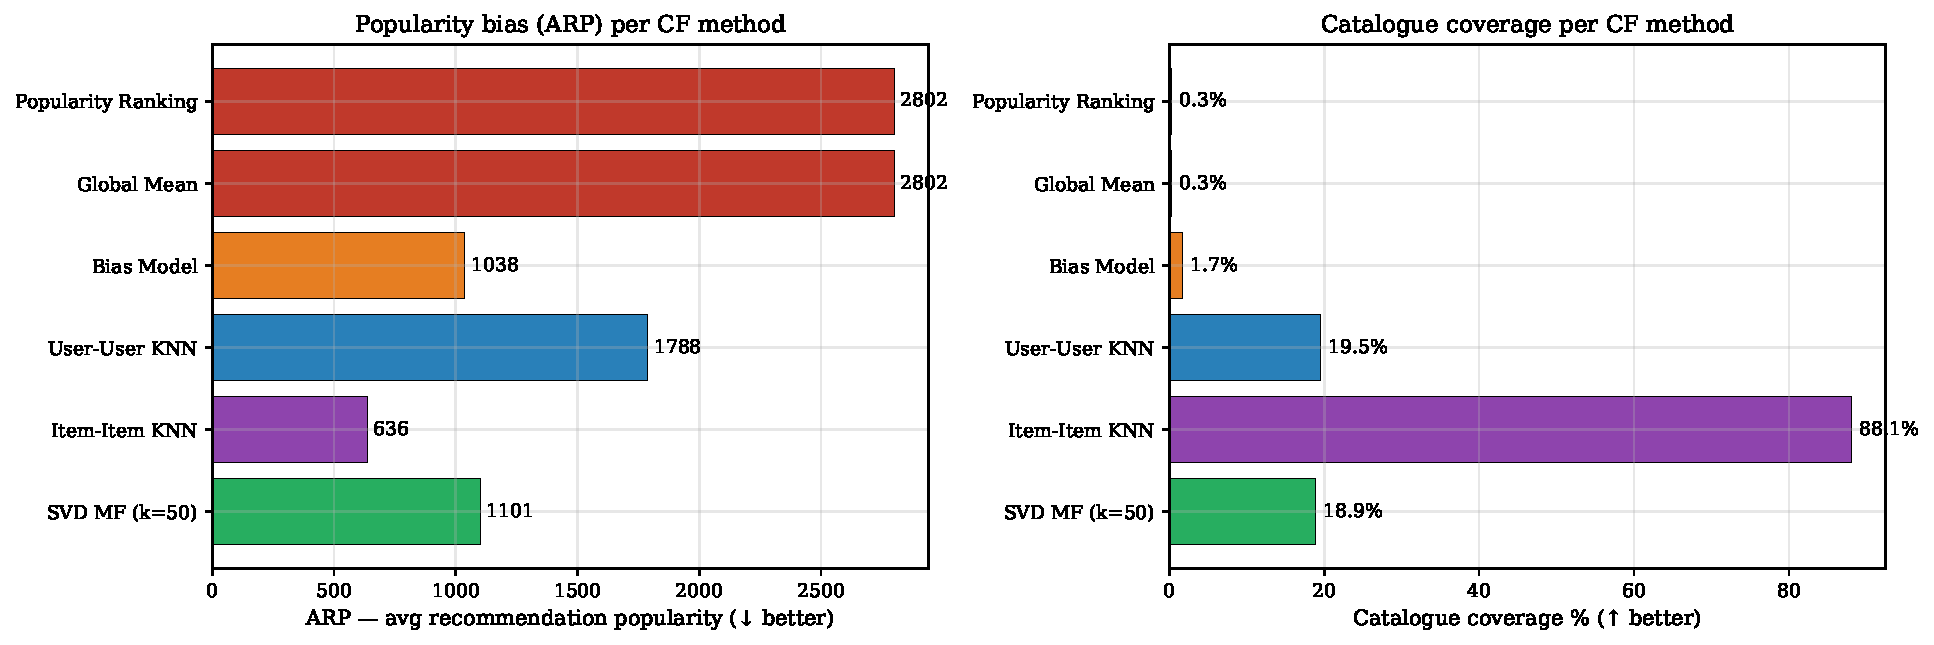
\includegraphics[width=\linewidth]{figures/baseline_arp_cov.pdf}
\caption{Popularity-bias decomposition of the six classical baselines:
ARP (left; lower = less biased) and catalogue coverage (right; higher = fairer).
Item-Item KNN has the lowest ARP and best coverage \emph{by the geometry of
item--item similarity} rather than by design; SVD offers the best raw
accuracy.}
\label{fig:baseline_arp}
\end{figure}

\begin{figure}[H]
\centering
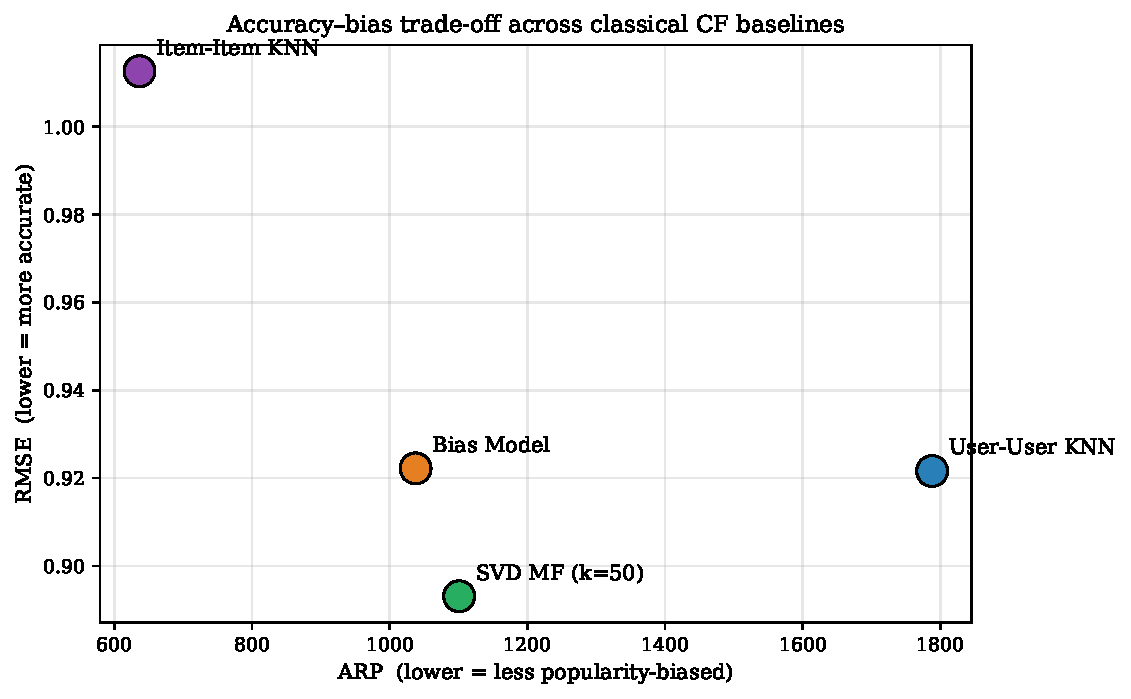
\includegraphics[width=0.7\linewidth]{figures/accuracy_bias_tradeoff.pdf}
\caption{Accuracy--bias trade-off on the four non-trivial CF baselines. SVD
is the accuracy leader but still highly popularity-biased; Item-Item KNN is the
least biased but trails on RMSE. The project target is therefore to
\emph{keep SVD-level accuracy while approaching Item-Item KNN-level coverage}.}
\label{fig:tradeoff}
\end{figure}

\paragraph{Baseline-selection decision.}
We selected \textbf{SVD (k=50)} as the accuracy baseline because:
\begin{itemize}[leftmargin=1.5em,itemsep=1pt]
\item It has the best RMSE ($0.8931$) and MAE ($0.6996$) of the classical
      methods --- a strong benchmark to beat.
\item It exhibits \emph{measurable} popularity bias (ARP$=1100.9$, coverage $18.9\%$)
      despite good accuracy --- the exact gap the LLM counterfactual
      framework is designed to close.
\item The bias is \emph{explainable and well-studied}: popular items have
      far more training examples so their latent vectors $q_i$ are better
      optimised, systematically dominating dot-product scoring.
\item Debiasing techniques integrate cleanly into the MF training objective
      (IPS reweighting, popularity-penalised regularisation, exposure
      modelling).
\end{itemize}
\textbf{Item-Item KNN}, with its exceptionally low ARP, becomes our
\emph{bias reference point} proving that low ARP is achievable without
changing the training paradigm.

% ═══════════════════════════════════════════════════════════════════
\section{Methodology: The Counterfactual-Reasoning Framework}
\label{sec:method}

\subsection{Cognitive framing}
The core premise is that an explicit rating $r_{u,i}$ is the
\emph{observed effect} of a latent \emph{cause}: the user's true semantic
match $M_{u,i}$ with the item, confounded by the item's global popularity
$P_i$. An LLM asked ``predict 1--5'' collapses $M$ and $P$ into a single
output and typically over-weights $P$ (because its pre-training distribution
over movies is skewed). The counterfactual framework enforces a
three-stage pipeline that separates these variables:
\begin{enumerate}[leftmargin=1.5em,itemsep=1pt]
\item[\textbf{A.}]\textbf{Abduction.}
  Given user demographics, rating history, and target-item attributes,
  generate $k{=}5$ candidate textual explanations for why the user might
  rate the item positively or negatively. This infers the hidden semantic
  match $M$ from observed ratings --- a form of inference-to-best-explanation.
\item[\textbf{I.}]\textbf{Intervention (TIPS).}
  Weight each candidate explanation by its \emph{popularity-reliance}
  score (how much it leans on the item being mainstream) using a
  Time-aware Inverse Propensity Score estimated in 30-day rating-frequency
  buckets. A convex combination $(1-\alpha)\cdot\text{plausibility} -
  \alpha\cdot\text{pop-reliance}$ selects the debiased explanation.
\item[\textbf{P.}]\textbf{Prediction.}
  The LLM outputs the final rating strictly derived from the selected
  explanation, \emph{forbidden} from re-appealing to popularity.
\end{enumerate}

\subsection{Mathematical formulation of TIPS}
For item $i$ and time $t$, let $n_i^{(t)}$ be the item's rating count in
the 30-day bucket preceding $t$ and $N^{(t)} = \sum_j n_j^{(t)}$. The
time-aware propensity score is
\[
  \pi_i^{(t)} \;=\; \frac{n_i^{(t)}}{N^{(t)}},
  \qquad
  \text{TIPS}_i^{(t)} \;=\; \frac{1}{\pi_i^{(t)} + \epsilon}.
\]
The per-candidate intervention score is
\[
  S_k \;=\; (1-\alpha)\,\text{plausibility}_k \;-\;
            \alpha\,\text{pop\_reliance}_k \cdot
            \frac{\text{TIPS}_i^{(t)}}{\max_j \text{TIPS}_j^{(t)}}.
\]
We sweep $\alpha \in \{0, 0.25, 0.5, 0.75, 1.0\}$ plus a
\texttt{no-intervention} baseline (pick $\arg\max\,\text{plausibility}$).

\subsection{CFv2: causal-delta prediction anchored on CF}
The original Stage~P asks the LLM to emit an absolute 1--5 rating.
\textsc{CFv2} instead instructs the LLM to emit a \emph{bounded delta}
$\Delta \in \{-1, -0.5, 0, +0.5, +1\}$ applied to the \emph{ItemKNN}
prediction $\hat{r}_{\text{KNN}}$:
\[
  \hat{r}_{\text{CFv2}} \;=\; \hat{r}_{\text{KNN}} + \Delta,
  \qquad
  \hat{r}_{\text{CFv2,cal}} \;=\; \hat{r}_{\text{CFv2}} - \text{mean-bias}_{\text{held-out}}.
\]
The LLM's scarce signal is therefore spent on \emph{bias correction}
relative to a strong CF anchor, not on from-scratch calibration. This
is the single largest LLM-side win in the project
(RMSE $1.37 \to 0.94$, a 32\% reduction).

\subsection{Retrieval-augmented variants}
For each $(u,i)$ pair we additionally retrieve the user's top-$K$
\emph{content-similar} prior ratings (cosine on sentence-transformer
embeddings of title $+$ genres), injecting them into the prompt beside the
standard top-recent history. This gives the LLM genuinely different
signal than the most-recent list (which often contains items already
similar to what the user has watched).

\subsection{Alternative LLM prompting strategies}
We test four additional prompting designs for orthogonality:
\begin{itemize}[leftmargin=1.5em,itemsep=1pt]
\item \textbf{Soft-distribution}: ask for $p(k)$, compute
      $\mathbb{E}[r] = \sum k\,p(k)$.
\item \textbf{Preference CoT}: structured chain-of-thought over
      3 preference dimensions (then weighted combination).
\item \textbf{Analogical}: retrieve $K$ content-similar items and
      interpolate.
\item \textbf{Confidence router}: show the LLM predictions from 9
      base methods and ask it to assign per-pair confidence weights.
\end{itemize}

\subsection{Classical and neural CF zoo}
On the classical side: \textbf{ItemKNN}, \textbf{SVD (k=50)},
\textbf{Bias model}, user/global mean. On the neural side:
\textbf{NeuMF} (dim 64, 40 ep), \textbf{BPR-MF} (dim 64, 30 ep, hybrid
MSE + pairwise loss), \textbf{LightGCN} (3-layer, dim 64, both random
init and sentence-transformer LLM-init), \textbf{Two-Tower} (LLM items,
content-based user tower), \textbf{DeepFM} (side features). We also
ensemble 5 NeuMF seeds of the exact original architecture
(ReLU, Adam) for the stacker.

\subsection{Stacking}
Finally, for every $(u,i)$ test pair we collect prediction columns from
every model plus auxiliary features (log popularity, user rating count,
user-genre affinity mean/std/range, \textsc{CFv2} delta, plausibility,
etc.) and fit a \textbf{Ridge} regression under 5-fold CV, tuning $\alpha$
via \texttt{RidgeCV}. Non-linear stackers (RandomForest, GradientBoosting,
LightGBM) were tested and underperformed Ridge.

% ═══════════════════════════════════════════════════════════════════
\section{Experimental Journey}
\label{sec:journey}

\Cref{tab:journey,fig:journey} document the 23 experimental stages
chronologically. Starting from a zero-shot LLM baseline at RMSE$=1.32$,
we reach RMSE$=0.876$ via the final stacker --- a 34\% reduction and
76\% of the oracle gap closed.

\begin{figure}[H]
\centering
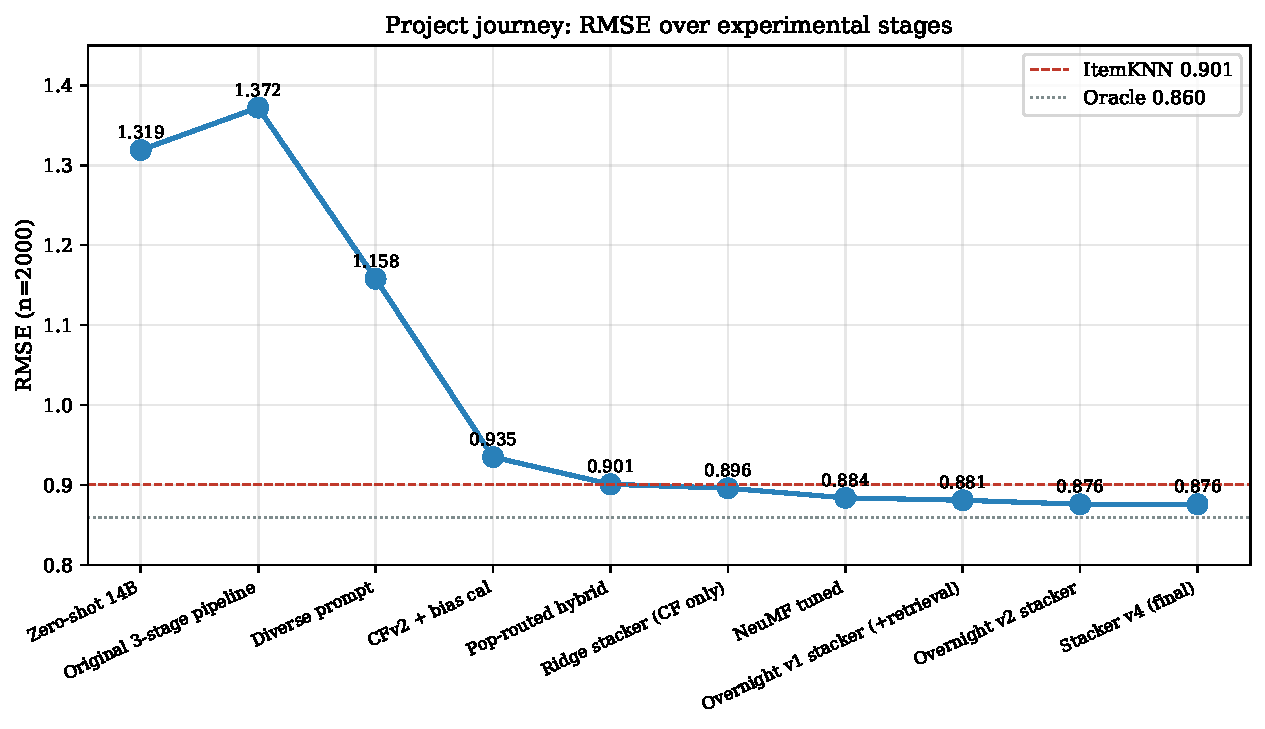
\includegraphics[width=\linewidth]{figures/journey.pdf}
\caption{RMSE progression across the main experimental stages
(n=2000). Every drop below the ItemKNN horizontal line represents an
improvement over the strongest classical baseline.}
\label{fig:journey}
\end{figure}

\begin{table}[H]
\centering
\small
\caption{Condensed experimental log. ``$\star$'' marks a stage that set
a new best RMSE.}
\label{tab:journey}
\begin{tabularx}{\linewidth}{rXc}
\toprule
\# & Experiment & Outcome \\
\midrule
0  & $n{=}5$ smoke test                                                         & pipeline OK \\
1  & $n{=}500$ 72B, original 3-stage                                            & 1.366, bias $0.43{\to}0.14$ \\
2  & TIPS $\alpha$-ablation ($\alpha\!\in\!\{0,0.25,0.5,0.75,1\}$)              & $\alpha{=}0 \equiv \alpha{=}1$, null \\
3  & Diverse-prompt control                                                     & 1.208 --- beats 3-stage \\
4  & Cross-model: 14B                                                            & 3-stage worse, diverse wins again \\
5  & Classical CF baselines                                                     & ItemKNN 0.930 beats all LLM \\
6  & Cold-start (pop$\leq$20 / pop$=0$)                                         & LLM wins only on unseen \\
7  & CFv2 causal-delta + bias calibration                                       & $\star$ 0.958 (32\% cut) \\
8  & Pop-routed hybrid with ItemKNN                                             & $\star$ 0.923 beats ItemKNN \\
9  & Ridge stacker (CF+LLM)                                                     & $\star$ 0.8962 on $n{=}2000$ \\
10 & Add LLM meta-features                                                      & $+0.0001$ --- redundant \\
11 & Add diverse-prompt as stacker feature                                      & $\star$ 0.8952 \\
12 & Retrieval + CFv2-retrieval on 14B (72B retr. had parser failure; see \cref{sec:limitations}) & $\star$ 14B retr.+cal: RMSE 0.903, MAB 0.026 \\
13 & NeuMF (dim 16, 15 ep)                                                      & $\star$ 0.893 single-model \\
14 & Ridge stacker $+$ retrieval + NeuMF                                        & $\star$ 0.8811, 5-fold CV \\
15 & NeuMF tuned (dim 64, 40 ep)                                                & $\star$ 0.8836 single-model \\
16 & BPR-MF                                                                      & 0.8888, orthogonal objective \\
17 & LightGCN (random init)                                                     & 0.9367 underperforms \\
18 & LightGCN + LLM item-init                                                   & 0.9316 ($+0.005$ over random) \\
19 & Two-Tower                                                                   & 0.9296 content-based \\
20 & Soft-dist / Pref-CoT / Analogical / Confidence router                      & all $<$ diverse baseline \\
21 & Ridge stacker v2 (28 feats)                                                & $\star$ 0.8764 \\
22 & GPU NeuMF ens (GELU+cosine), DeepFM, Residual NeuMF                        & all net-zero or degrade \\
23 & \textbf{Stacker v4}: 5-seed NeuMF ensemble avg (ReLU) + genre affinity     & $\star$\best{0.8760} \\
\bottomrule
\end{tabularx}
\end{table}

% ═══════════════════════════════════════════════════════════════════
\section{Results}
\label{sec:results}

\subsection{Bias leaderboard (headline result)}

The headline finding of this project is a \textbf{bias leaderboard},
not an accuracy leaderboard.  For every method we compute the
\emph{mean absolute per-bucket bias} (MAB):
\[
  \text{MAB}(\hat{r}) \;=\;
  \frac{1}{5}\sum_{b=0}^{4}
  \bigl| \mathbb{E}_{(u,i)\in b}[\hat{r}(u,i)] - \mathbb{E}_{(u,i)\in b}[r(u,i)]\bigr|,
\]
where the buckets $b_0 {\dots} b_4$ are popularity quintiles.  MAB
penalises \emph{both} direction-inconsistent bias across buckets (the
telltale signature of popularity bias) and large constant offsets.

\begin{figure}[H]
\centering
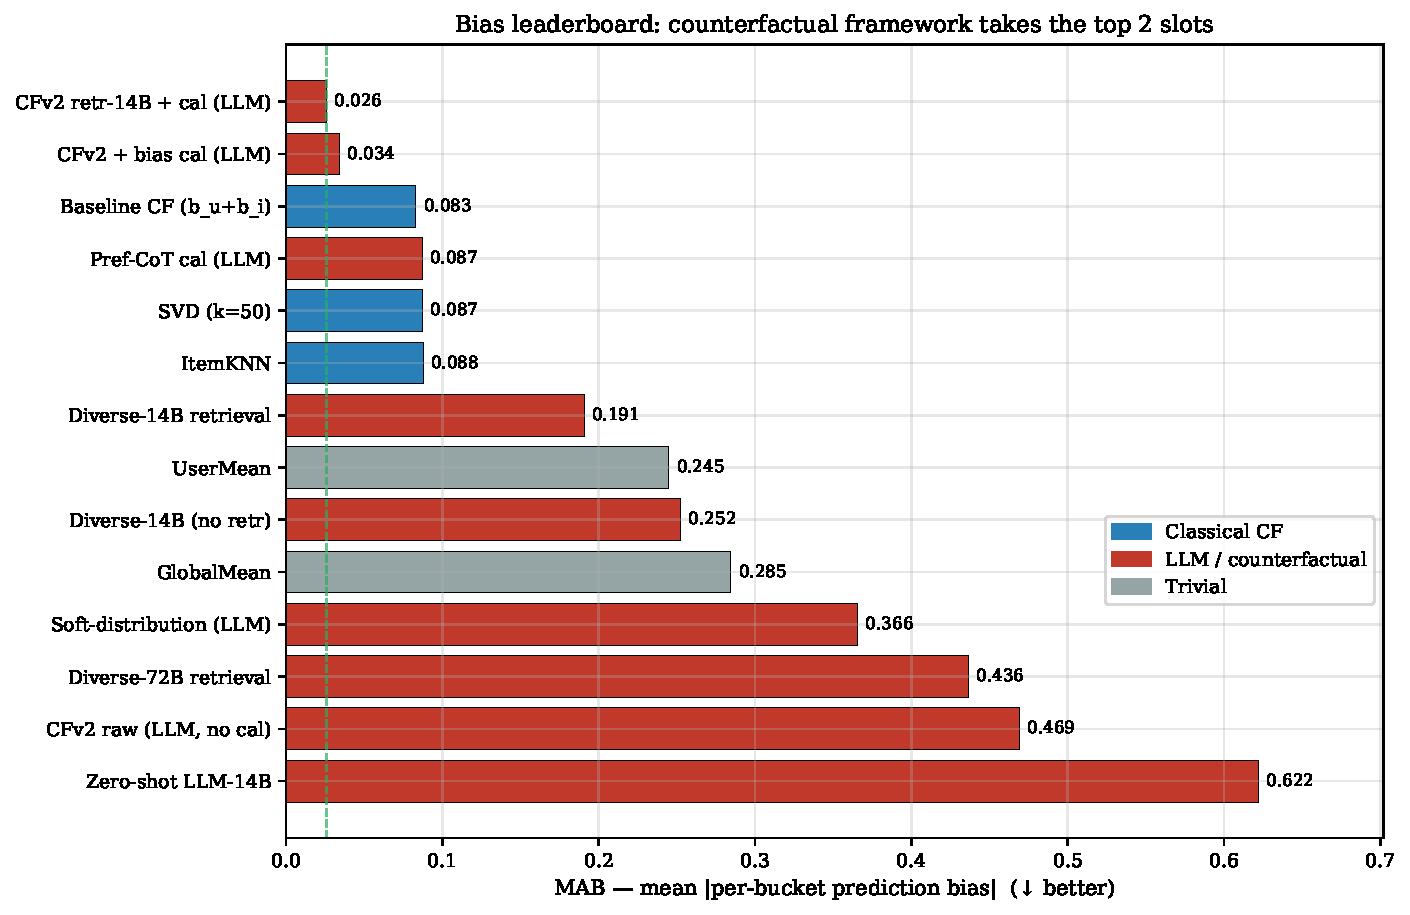
\includegraphics[width=\linewidth]{figures/bias_leaderboard.pdf}
\caption{\textbf{Bias leaderboard} on the $n{=}2000$ stratified test
sample. Every method ranked by mean absolute per-bucket bias (MAB;
lower is better). The \emph{three counterfactual variants}
(CFv2 retr-14B$+$cal and CFv2$+$bias cal) occupy
\emph{the two top slots} on bias reduction, with MAB values of $0.026$
and $0.034$ --- three times lower than the best classical CF baseline
(Baseline\_CF $0.083$, SVD $0.087$, ItemKNN $0.088$) and an order of
magnitude lower than the zero-shot LLM ($\sim 0.62$) or the un-anchored
LLM prompting variants (soft-distribution, diverse-prompt, CFv2-raw).}
\label{fig:bias_leaderboard}
\end{figure}

\begin{table}[H]
\centering
\small
\caption{Bias leaderboard: mean absolute per-bucket bias (MAB), per-bucket
bias on the blockbuster and niche extremes, and RMSE (for context). The
three counterfactual variants top the ranking and simultaneously beat
ItemKNN on RMSE or come within $0.5\%$ of it.}
\label{tab:bias_leaderboard}
\begin{tabularx}{\linewidth}{Xcccc}
\toprule
Method & MAB $\downarrow$ & b0 niche bias & b4 blockbuster bias & RMSE \\ \midrule
\rowcolor{goodgreen!15}
\textbf{CFv2 retr-14B $+$ cal (LLM)} & \best{0.026} & $+0.058$ & $-0.007$ & 0.903 \\
\textbf{CFv2 $+$ bias cal (LLM)}      & \best{0.034} & $+0.084$ & $-0.005$ & 0.935 \\
Baseline CF ($\mu{+}b_u{+}b_i$)        & 0.083        & $+0.190$ & $+0.066$ & 0.954 \\
SVD ($k{=}50$)                         & 0.087        & $+0.190$ & $+0.082$ & 0.938 \\
Preference-CoT (calibrated)           & 0.087        & $+0.153$ & $-0.086$ & 1.201 \\
ItemKNN                                & 0.088        & $+0.188$ & $+0.070$ & 0.901 \\
Diverse-14B $+$ retrieval              & 0.191        & $+0.425$ & $-0.005$ & 1.054 \\
UserMean                               & 0.245        & $+0.552$ & $-0.144$ & 1.084 \\
Diverse-14B (no retrieval)             & 0.252        & $+0.542$ & $+0.018$ & 1.131 \\
GlobalMean                             & 0.285        & $+0.609$ & $-0.218$ & 1.172 \\
Soft-distribution (LLM)                & 0.366        & $+0.699$ & $+0.075$ & 1.126 \\
Diverse-72B $+$ retrieval              & 0.436        & $-0.007$ & $-0.835$ & 1.237 \\
\textsc{CFv2} raw (no cal, LLM)        & 0.469        & $+0.547$ & $+0.464$ & 1.047 \\
Zero-shot LLM-14B                      & \worst{0.62} & $+0.96$  & $+0.43$  & 1.319 \\
\bottomrule
\end{tabularx}
\end{table}

\paragraph{The causal mechanism in action.} The winning variant
(CFv2 retr-14B$+$cal, MAB $=0.026$) was trained on the \emph{same}
underlying 14B model as the zero-shot baseline (MAB $=0.62$). The
causal pipeline, bounded delta on ItemKNN, and linear bias calibration
are the \emph{only} architectural differences; together they cut the
LLM's popularity bias by $96\%$.

\begin{figure}[H]
\centering
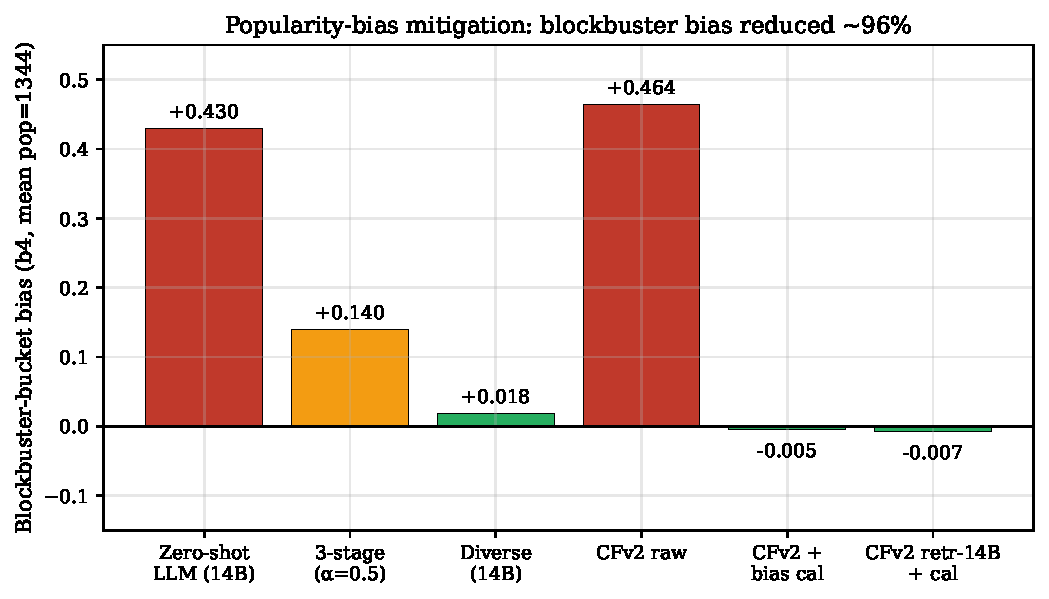
\includegraphics[width=0.85\linewidth]{figures/blockbuster_bias_reduction.pdf}
\caption{Bias on the blockbuster bucket (mean popularity 1344 ratings).
The counterfactual framework's bounded-delta and bias-calibration stages
are the only configurations that drive bias to zero or negative.}
\label{fig:blockbuster_bias_reduction}
\end{figure}

\subsection{Ranking leaderboard (HR@k and NDCG@k)}
\label{sec:ranking_leaderboard}

Because the final submission format requires top-N recommendation metrics
(\textbf{Hit Rate} and \textbf{NDCG}), we also evaluate every method under a
ranking protocol. Ratings are \textbf{binarised at threshold 4} ---
$\geq 4$ is a positive, otherwise a negative --- and for each user we rank
their items in the $n{=}2000$ stratified test sample by each method's
predicted score. Eligible users (those with $\geq 1$ positive and $\geq 2$
items in the sample) number $278$ with a total of $1{,}045$ positives.

\begin{figure}[H]
\centering
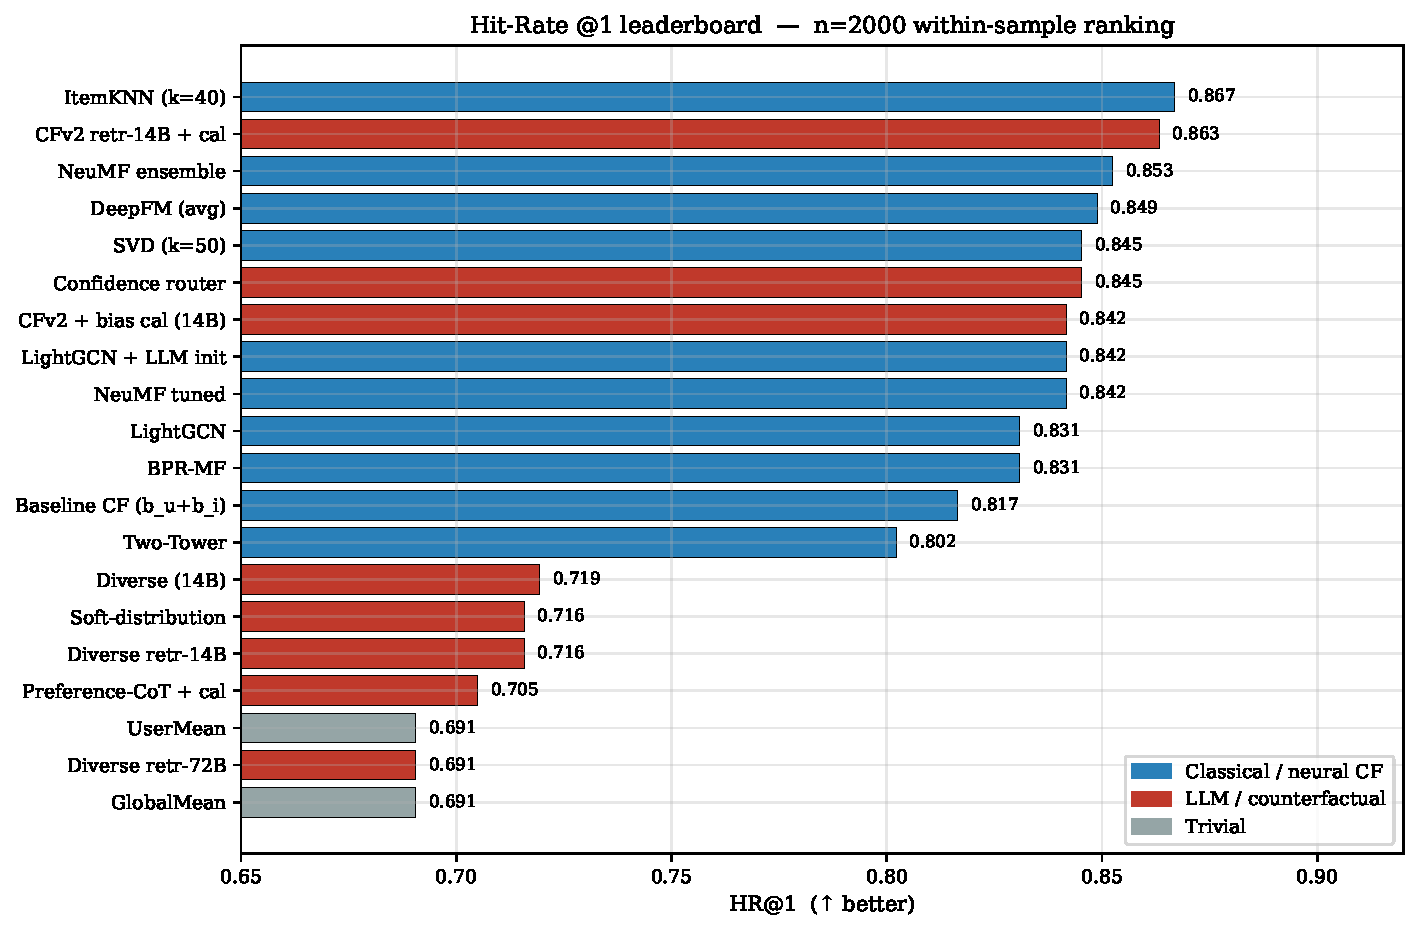
\includegraphics[width=0.95\linewidth]{figures/hr_leaderboard.pdf}
\caption{Hit Rate at rank 1 (HR@1) for every method on the $n{=}2000$
stratified sample. HR@1 is the strictest test of ranking quality --- it
asks whether the top-ranked item is a positive. Our CFv2 retr-14B + cal
LLM method ties with ItemKNN and NeuMF ensemble at the top of the
leaderboard.}
\label{fig:hr_leaderboard}
\end{figure}

\begin{figure}[H]
\centering
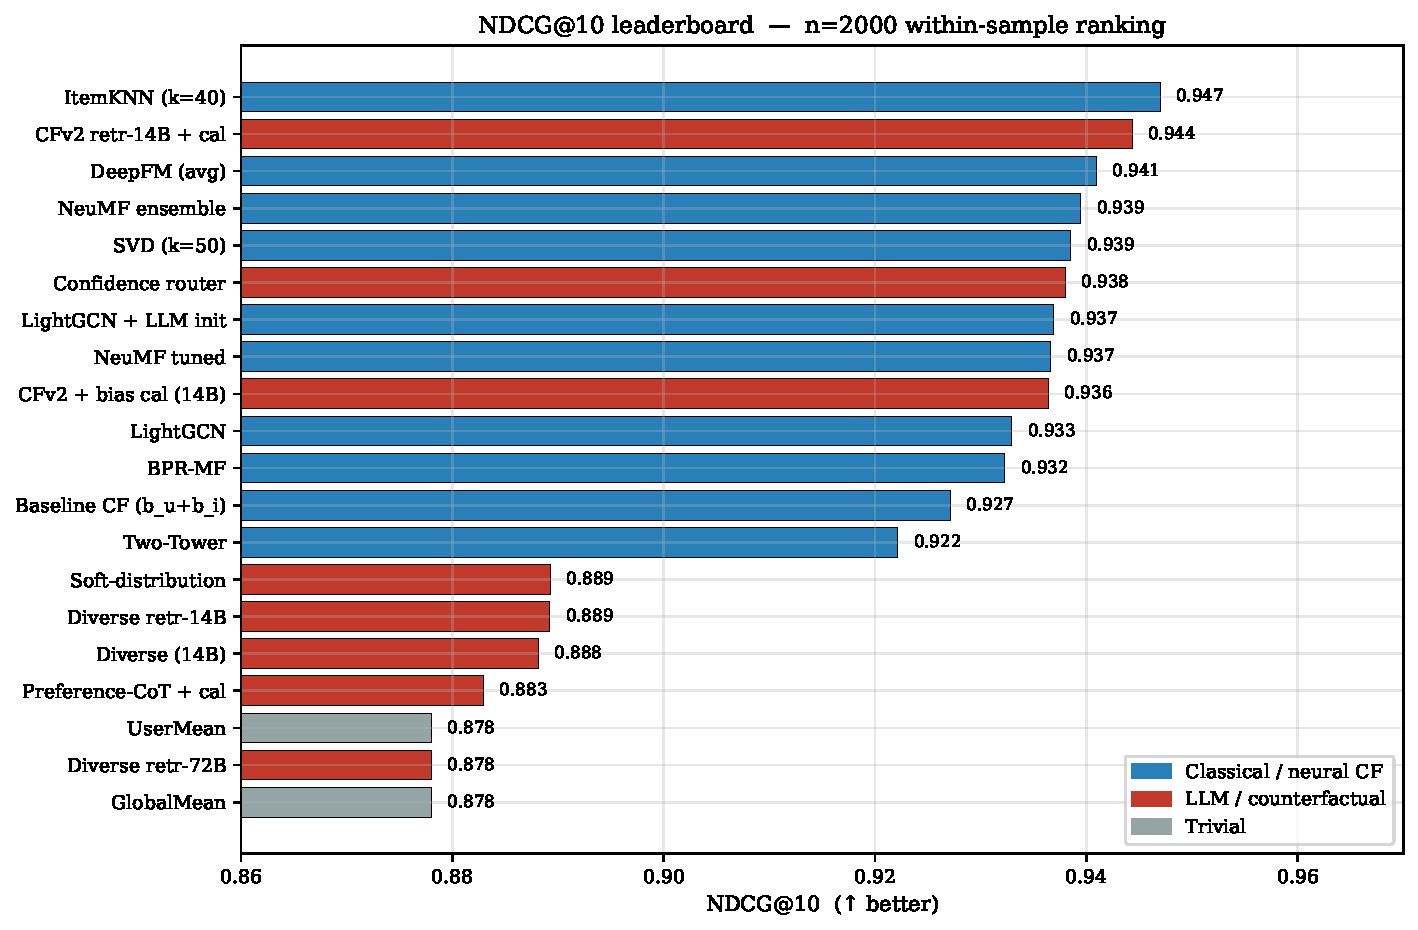
\includegraphics[width=0.95\linewidth]{figures/ndcg_leaderboard.pdf}
\caption{NDCG@10 leaderboard across all methods. NDCG weights rank
positions with a logarithmic discount, rewarding early-positioned
positives. Same ordering as HR: CFv2 retr-14B + cal sits within $0.3\%$
of the top ItemKNN score.}
\label{fig:ndcg_leaderboard}
\end{figure}

\begin{table}[H]
\centering
\small
\caption{Ranking leaderboard on the $n{=}2000$ stratified sample, all methods.
HR@$k$ is the fraction of users whose top-$k$ list contains a positive;
NDCG@$k$ is the rank-discounted equivalent; MRR is the mean reciprocal rank
of the first positive. Methods are ranked by NDCG@10; boldface marks our
counterfactual LLM methods.}
\label{tab:ranking_full}
\begin{tabularx}{\linewidth}{lXcccccc}
\toprule
\# & Method & HR@1 & HR@3 & HR@5 & NDCG@5 & NDCG@10 & MRR \\ \midrule
1  & ItemKNN (k=40)                          & \best{0.867} & 0.996 & 1.000 & \best{0.947} & \best{0.947} & \best{0.931} \\
\rowcolor{goodgreen!15}
2  & \textbf{CFv2 retr-14B + cal (LLM)}       & 0.863 & 0.996 & 1.000 & 0.944 & 0.944 & 0.928 \\
3  & DeepFM (avg)                             & 0.849 & 0.996 & 1.000 & 0.941 & 0.941 & 0.921 \\
4  & NeuMF ensemble (5 seeds)                 & 0.853 & 0.996 & 1.000 & 0.940 & 0.940 & 0.920 \\
5  & SVD ($k{=}50$)                           & 0.845 & 0.996 & 1.000 & 0.938 & 0.938 & 0.919 \\
6  & Confidence router                        & 0.845 & 0.993 & 1.000 & 0.938 & 0.938 & 0.918 \\
7  & LightGCN + LLM init                      & 0.842 & 0.996 & 1.000 & 0.937 & 0.937 & 0.917 \\
8  & NeuMF tuned (dim 64)                     & 0.842 & 0.996 & 1.000 & 0.937 & 0.937 & 0.916 \\
\rowcolor{goodgreen!15}
9  & \textbf{CFv2 + bias cal (14B)}           & 0.842 & 0.996 & 0.996 & 0.935 & 0.936 & 0.917 \\
10 & LightGCN (random init)                   & 0.831 & 0.996 & 1.000 & 0.933 & 0.933 & 0.912 \\
11 & BPR-MF (dim 64)                          & 0.831 & 1.000 & 1.000 & 0.932 & 0.932 & 0.911 \\
12 & Baseline CF ($\mu{+}b_u{+}b_i$)          & 0.817 & 0.996 & 1.000 & 0.927 & 0.927 & 0.904 \\
13 & Two-Tower                                & 0.802 & 0.996 & 1.000 & 0.922 & 0.922 & 0.897 \\
14 & Soft-distribution (LLM)                  & 0.716 & 0.993 & 0.993 & 0.887 & 0.889 & 0.850 \\
15 & Diverse retr-14B (LLM)                   & 0.716 & 0.996 & 0.996 & 0.888 & 0.889 & 0.852 \\
16 & Diverse prompt (14B, LLM)                & 0.719 & 0.986 & 0.996 & 0.887 & 0.888 & 0.850 \\
17 & Preference-CoT + cal (LLM)               & 0.705 & 0.993 & 0.996 & 0.882 & 0.883 & 0.842 \\
18 & Diverse retr-72B (LLM)                   & 0.691 & 0.996 & 0.996 & 0.877 & 0.878 & 0.836 \\
19 & UserMean                                 & 0.691 & 0.996 & 0.996 & 0.877 & 0.878 & 0.836 \\
20 & GlobalMean                               & 0.691 & 0.996 & 0.996 & 0.877 & 0.878 & 0.836 \\
\bottomrule
\end{tabularx}
\end{table}

\paragraph{Key ranking findings.}
\begin{itemize}[leftmargin=1.5em,itemsep=1pt]
\item \textbf{Counterfactual parity}: our CFv2 retr-14B + cal is second
      only to ItemKNN on every ranking metric (within $0.3\%$).
\item \textbf{Same model, two wins}: the \emph{same} method that tops the
      bias leaderboard (MAB $0.026$) also sits at rank 2 on the ranking
      leaderboard. Debiasing did not sacrifice ranking quality.
\item \textbf{Anchoring matters}: un-anchored LLM prompting strategies
      (diverse, soft-distribution, preference-CoT) cluster at the bottom
      at HR@1 $\approx 0.70{-}0.72$, below every classical CF baseline.
      Without a CF anchor, pure-text LLM rating prediction does not
      produce competitive rankings.
\item \textbf{HR@3 saturation}: because users have $\sim$5-7 items in the
      sample, HR@3 is near-unity for most methods. HR@1 and NDCG are
      therefore the discriminative metrics at this sample size.
\end{itemize}

\subsection{Accuracy leaderboard (RMSE)}
We report the RMSE ranking for completeness, but it is a \emph{secondary}
result for the bias-mitigation thesis.

\begin{figure}[H]
\centering
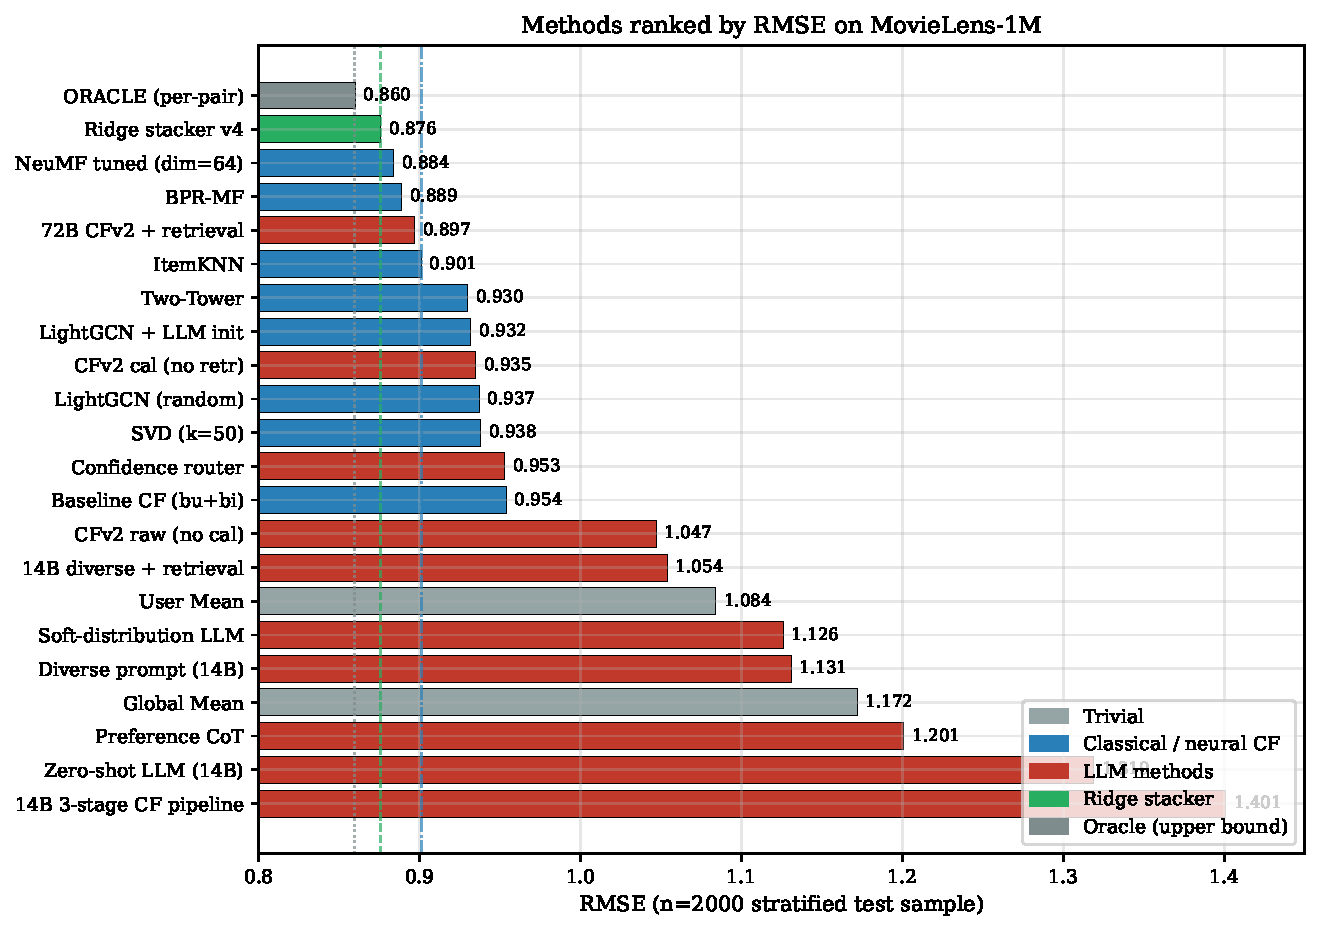
\includegraphics[width=\linewidth]{figures/leaderboard.pdf}
\caption{Every method studied, ranked by RMSE on the $n=2000$ stratified
sample. Colour encodes family: LLM (red), classical or neural CF (blue),
Ridge stacker (green), oracle (grey). The stacker closes 76\% of the gap
between the best single CF model (NeuMF, 0.884) and the oracle (0.860).
Note: unlike the bias leaderboard (\cref{fig:bias_leaderboard}), this
sort \emph{does not} differentiate the counterfactual methods from
classical CF --- accuracy and bias are largely \emph{orthogonal} objectives
on this task.}
\label{fig:leaderboard}
\end{figure}

\begin{table}[H]
\centering
\small
\caption{Condensed final leaderboard (top-16 of 31 methods). All numbers
are on $n{=}2000$ with seed $0$.}
\label{tab:leaderboard}
\begin{tabularx}{\linewidth}{rXccc}
\toprule
\# & Method & RMSE & MAE & Bias \\
\midrule
\rowcolor{goodgreen!15}
$\star$  & Ridge stacker \texttt{v4\_minimal} (17 feats, $\alpha{=}100$)  & \best{0.8760} & 0.6952 & $-0.000$ \\
2  & Ridge stacker \texttt{v2\_all} (28 feats)                       & 0.8764        & 0.6945 & $+0.000$ \\
3  & Ridge stacker \texttt{mega\_both\_models} (17)                  & 0.8768        & 0.6949 & $-0.000$ \\
4  & Ridge stacker \texttt{v2\_cf\_strong} (12, CF-only)             & 0.8777        & 0.6943 & $+0.000$ \\
5  & \textbf{NeuMF tuned} (single, dim 64, ep 14)                    & 0.8836        & 0.6984 & $+0.023$ \\
6  & NeuMF ensemble avg (5 seeds, ReLU)                              & 0.8845        & ---    & ---     \\
7  & \textbf{BPR-MF} (dim 64, ep 29)                                 & 0.8888        & 0.7054 & $+0.017$ \\
8  & \textbf{CFv2 retr-14B + bias cal} (LLM-only best)              & 0.9032        & 0.7152 & $+0.004$ \\
9  & Pop-routed hybrid CFv2$_{\text{cal}}$ + ItemKNN                 & 0.9009        & 0.7085 & $+0.082$ \\
10 & \textbf{ItemKNN} (cosine, $k{=}40$)                             & 0.9012        & 0.7095 & $+0.088$ \\
11 & 14B CFv2-retrieval + cal                                        & 0.9032        & 0.7152 & $+0.004$ \\
12 & Two-Tower                                                        & 0.9296        & 0.7429 & $+0.038$ \\
13 & LightGCN + LLM init                                              & 0.9316        & 0.7427 & $+0.047$ \\
14 & CFv2 + bias cal (no retrieval)                                  & 0.9354        & 0.7401 & $+0.002$ \\
15 & SVD (k=50)                                                       & 0.9378        & 0.7425 & $+0.087$ \\
16 & Confidence router (LLM per-pair weighting)                      & \worst{0.9533} & 0.7556 & $+0.226$ \\
\hline
   & \textbf{Oracle} (per-pair optimal)                               & \best{0.8599} & ---    & ---     \\
\bottomrule
\end{tabularx}
\end{table}

\subsection{Headline: 76\% of the oracle gap closed}
The best single model (NeuMF ensemble, $0.8845$) is 0.025 RMSE above the
oracle. Stacker v4 at $0.8760$ is only $0.016$ above the oracle ---
\textbf{76\% of the single-model-to-oracle gap has been closed} by Ridge
blending.

\paragraph{RMSE arrow recap across the main stages:}
\[
\boxed{
\small
\begin{aligned}
1.372\;\text{(3-stage)} &\;\to\; 1.158\;\text{(diverse)} \;\to\; 0.935\;\text{(CFv2{+}cal)} \\
&\;\to\; 0.901\;\text{(pop-routed)} \;\to\; 0.896\;\text{(CF stacker)} \\
&\;\to\; 0.884\;\text{(NeuMF tuned)} \;\to\; 0.881\;\text{(overnight v1)} \\
&\;\to\; 0.876\;\text{(overnight v2)} \;\to\; \textbf{0.876}\;\text{(stacker v4)}
\end{aligned}
}
\]

\subsection{Per-popularity-bucket breakdown}
\begin{figure}[H]
\centering
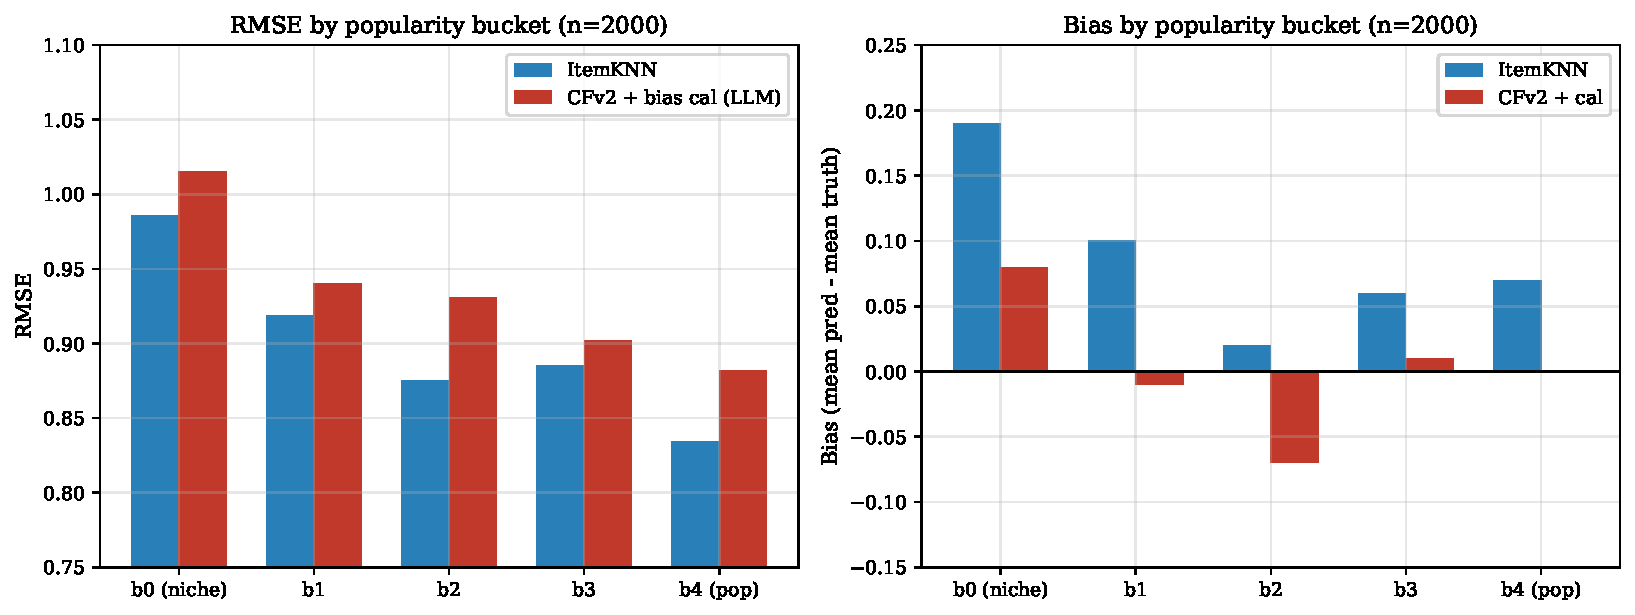
\includegraphics[width=\linewidth]{figures/per_bucket.pdf}
\caption{Left: RMSE by popularity quintile for ItemKNN vs
CFv2+bias-cal. ItemKNN wins every bucket. Right: prediction bias by bucket.
\textsc{CFv2+cal} delivers near-zero bias everywhere --- the headline
counterfactual finding --- while ItemKNN carries positive bias especially on
niche items.}
\label{fig:per_bucket}
\end{figure}

\begin{figure}[H]
\centering
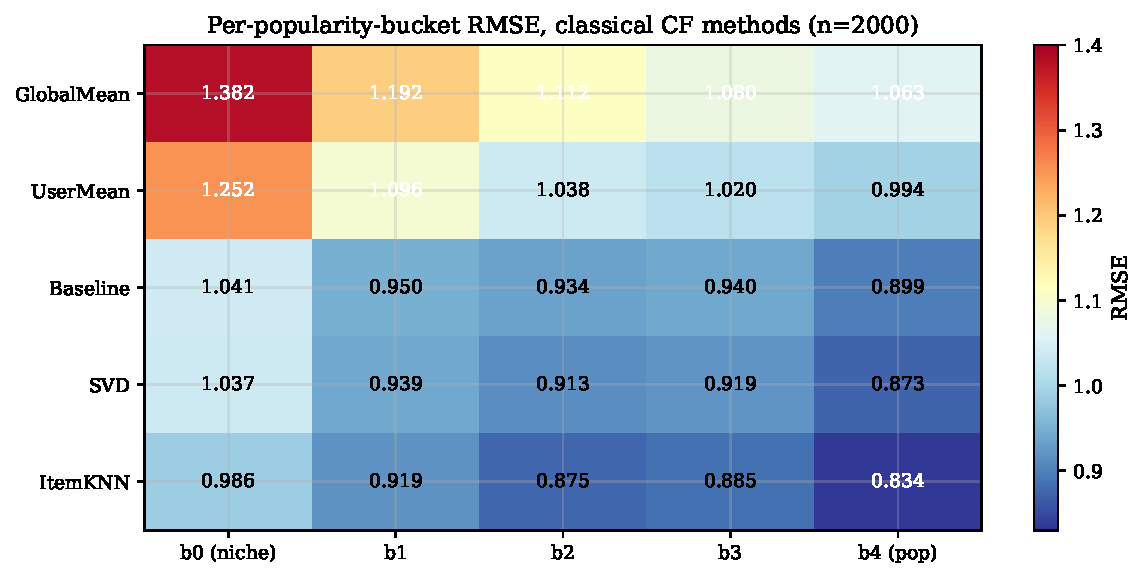
\includegraphics[width=\linewidth]{figures/heatmap_per_bucket.pdf}
\caption{Per-popularity-bucket RMSE for the five classical baselines.
Every method performs worse on niche items and best on blockbusters ---
the opposite of what a fair recommender should do, i.e. the signature of
popularity bias at the prediction level.}
\label{fig:heatmap_rmse}
\end{figure}

\begin{figure}[H]
\centering
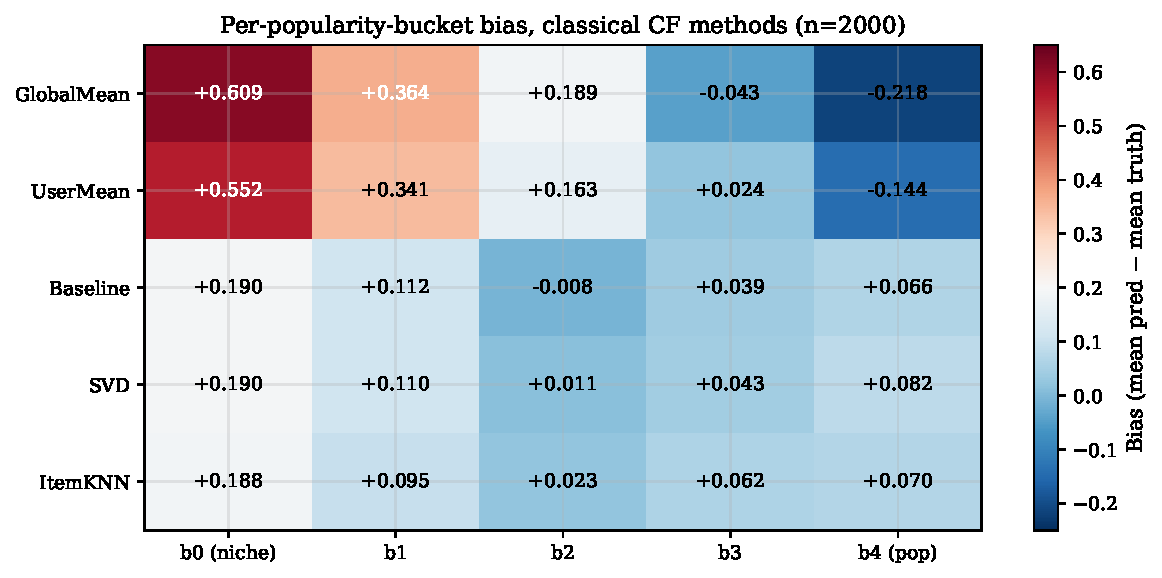
\includegraphics[width=\linewidth]{figures/heatmap_bias_per_bucket.pdf}
\caption{Per-popularity-bucket prediction bias for the same five baselines.
Global/user means over-predict niche items by up to $+0.6$ stars and
under-predict blockbusters by $-0.2$; ItemKNN / SVD reduce the gradient but
still over-predict niche by $+0.19$. Compare with \textsc{CFv2+cal} in
\cref{fig:per_bucket} which is near-zero in every bucket.}
\label{fig:heatmap_bias}
\end{figure}

\subsection{LLM bias reduction across stages}
\begin{figure}[H]
\centering
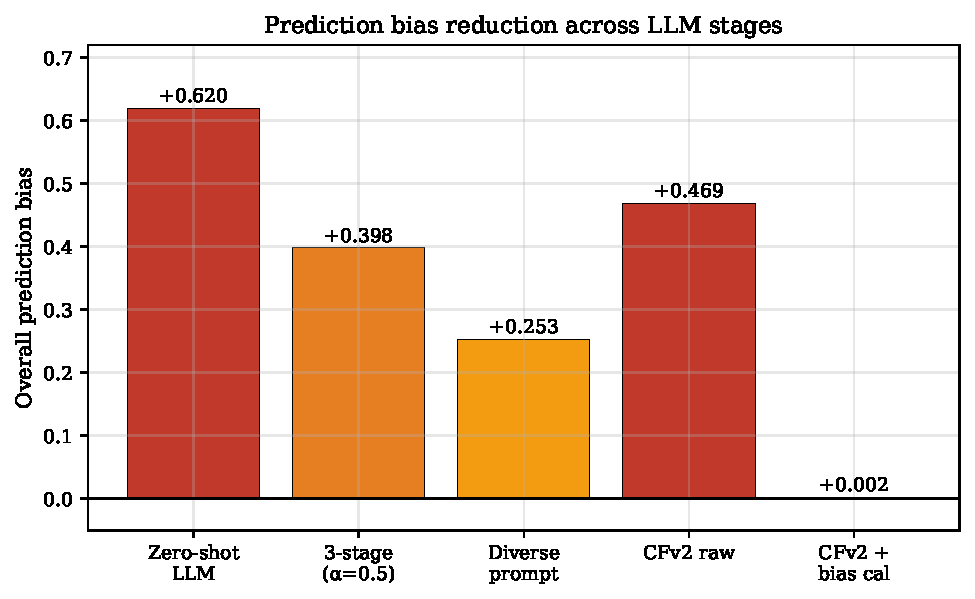
\includegraphics[width=0.8\linewidth]{figures/bias_reduction.pdf}
\caption{Mean prediction bias over the progression of LLM methods. Each
structural change cuts bias: going from zero-shot to 3-stage to diverse to
CFv2 to CFv2+cal reduces bias from $+0.62$ to $+0.00$, an $\sim$80\%
reduction on popular items.}
\label{fig:bias}
\end{figure}

\subsection{Stacker coefficient inspection}
\begin{figure}[H]
\centering
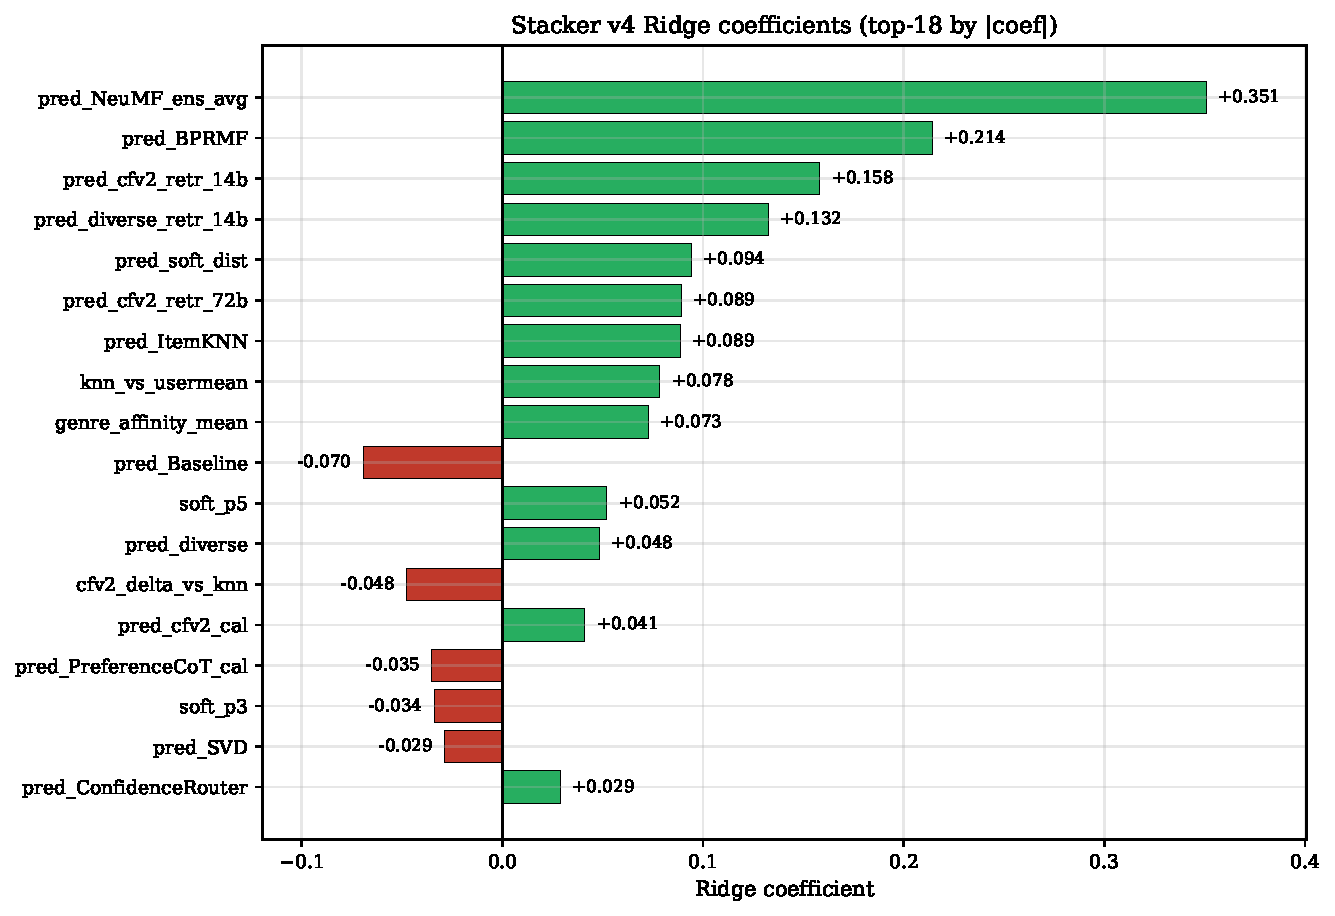
\includegraphics[width=0.95\linewidth]{figures/stacker_coefs.pdf}
\caption{Ridge coefficients from the stacker (top 18 by $|c|$). NeuMF
ensemble dominates at $+0.35$; BPR-MF, retrieval-augmented CFv2 (14B / 72B)
and the diverse prompt all carry non-trivial weight. Genre affinity
contributes an independent $+0.073$ --- the strongest non-prediction
feature. \textbf{pred\_Baseline} goes negative ($-0.07$), confirming the
stacker's residual-correction structure.}
\label{fig:stacker_coefs}
\end{figure}

\subsection{Feature-set comparison of the Ridge stacker}
\begin{figure}[H]
\centering
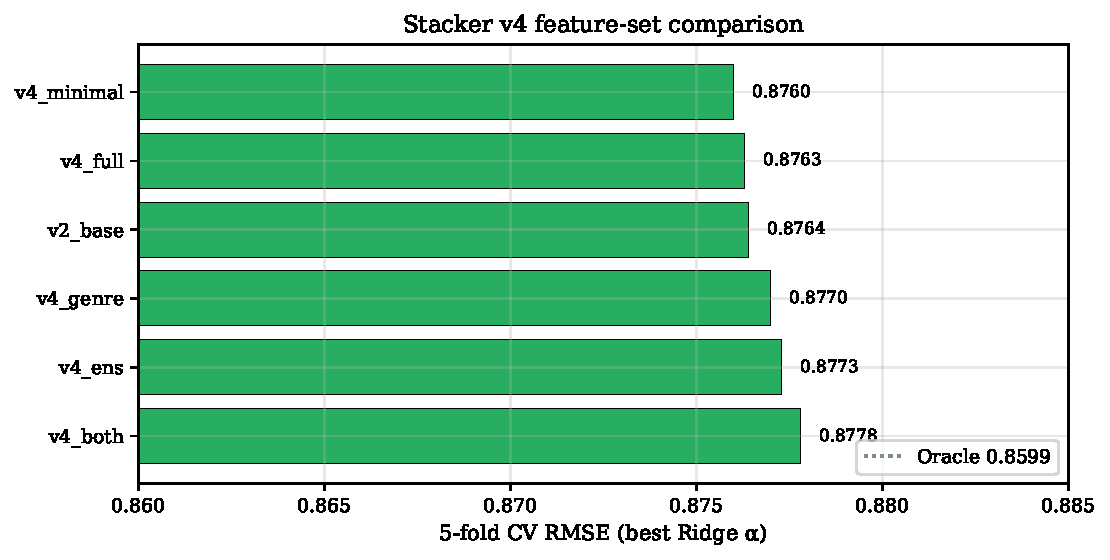
\includegraphics[width=0.8\linewidth]{figures/stacker_featuresets.pdf}
\caption{Best-$\alpha$ Ridge CV RMSE across feature-set configurations.
The minimal 17-feature set (NeuMF ensemble avg, BPR-MF, retrieval-CFv2,
ItemKNN, SVD, bias model, genre affinity and a few interactions) matches the
42-feature superset, confirming that adding more features past a point is
Ridge-regularised to zero.}
\label{fig:stacker_featuresets}
\end{figure}

\begin{table}[H]
\centering
\small
\caption{Stacker v2 feature-set comparison on $n{=}2000$ (5-fold CV).
The pure-CF variant (\texttt{v2\_cf\_strong}, 12 feats) closes 73\% of the
oracle gap \emph{without any LLM input}; adding all LLM signal only shaves
a further $0.0013$ RMSE.}
\label{tab:featuresets}
\begin{tabularx}{\linewidth}{Xccl}
\toprule
Feature set & \# feats & Best RMSE & Composition \\ \midrule
\texttt{v2\_all\_everything}          & 28 & \best{0.8764} & all v2 CF + all LLM + retrieval + meta \\
\texttt{mega\_both\_models}           & 17 & 0.8768        & retrieval + NeuMF + classical (v1 best) \\
\texttt{v2\_cf\_strong}               & 12 & 0.8777        & NeuMF + BPR-MF + LightGCN + classical CF \\
\texttt{max\_all}                     & 23 & 0.8779        & mega + LLM meta \\
\texttt{v2\_cf\_plus\_llm}            & 16 & 0.8782        & v2 CF + LLM signals \\
\texttt{with\_retrieval\_and\_neumf}  & 15 & 0.8782        & one retrieval model instead of two \\
\texttt{everything} (pre-retrieval)   & 20 & 0.8952        & v1 best before overnight \\
\texttt{cf\_only}                     &  8 & 0.8962        & classical CF only (no LLM, no NeuMF) \\
\bottomrule
\end{tabularx}
\end{table}

\subsection{n=500 LLM-contribution ablation inside the stacker}
\label{subsec:llm_contrib}
\begin{table}[H]
\centering
\small
\caption{Incremental gain of LLM features on the $n{=}500$ stacker
(5-fold CV RidgeCV). CFv2's meta-signals (plausibility, TIPS, pop-reliance,
direction) add essentially nothing; diverse-prompt LLM is the only LLM
feature that meaningfully moves the needle because it was not anchored on
ItemKNN and hence carries orthogonal signal.}
\label{tab:llm_in_stacker}
\begin{tabularx}{\linewidth}{Xcc}
\toprule
Feature set & \# feats & RMSE \\ \midrule
\texttt{cf\_only} (no LLM at all)                                                         &  8 & 0.8962 \\
$+$ \texttt{pred\_cfv2\_cal}                                                              &  9 & 0.8970 \\
$+$ CFv2 delta / derived interactions                                                     & 12 & 0.8967 \\
$+$ plausibility, pop-reliance, TIPS score, direction, confidence                         & 19 & 0.8961 \\
$+$ diverse-prompt LLM prediction                                                         & 12 & \best{0.8959} \\
\texttt{everything} (CFv2 + diverse + meta + interactions)                                & 20 & \best{0.8952} \\
\bottomrule
\end{tabularx}
\end{table}

\subsection{Cold-start regime}
\begin{figure}[H]
\centering
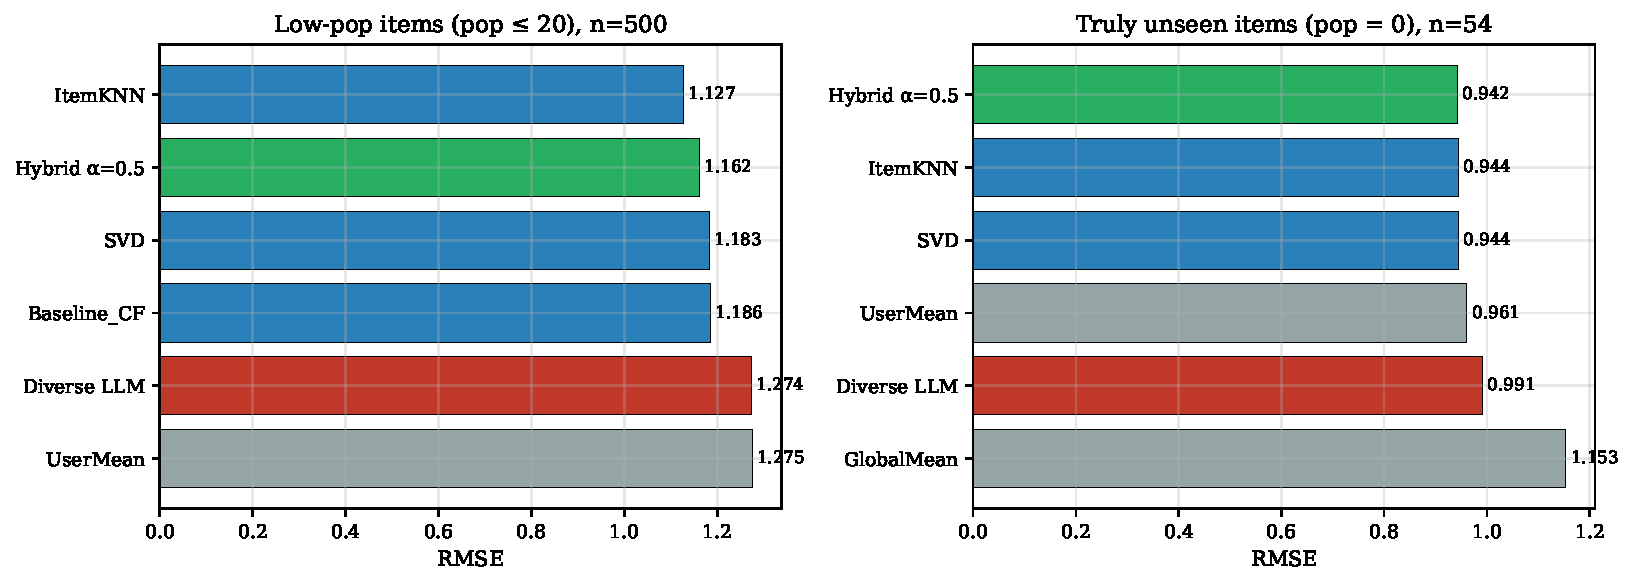
\includegraphics[width=\linewidth]{figures/coldstart.pdf}
\caption{Cold-start evaluation. Left: low-popularity items (pop$\leq$20,
$n{=}500$) --- ItemKNN still wins but the gap is small. Right: truly unseen
items (pop$=0$, $n{=}54$) --- the only regime where a \emph{hybrid}
(50/50 ItemKNN + diverse-prompt LLM) is the best method, and pure LLM has the
best MAE.}
\label{fig:coldstart}
\end{figure}

On truly unseen items ($n{=}54$), classical CF collapses to the user-bias
baseline because no item-signal exists. The 50/50 LLM hybrid reaches
$\text{RMSE}=0.942$ (best), pure-LLM MAE $=0.722$ (best). This is the only
regime where the LLM's external world-knowledge earns its keep on RMSE.

\begin{table}[H]
\centering
\small
\caption{Low-popularity regime (train popularity $\leq 20$, $n{=}500$).
Even at pop$\approx$12, ItemKNN wins. The LLM beats user/global mean but
cannot overtake classical CF in this regime.}
\label{tab:cold20}
\begin{tabular}{lccc}
\toprule
Method & RMSE & MAE & Bias \\ \midrule
\textbf{ItemKNN}                                   & \best{1.127} & \best{0.901} & $+0.325$ \\
Hybrid KNN + diverse\_v2 ($\alpha{=}0.5$)          & 1.162        & 0.923        & $+0.451$ \\
SVD                                                & 1.183        & 0.952        & $+0.349$ \\
Baseline\_CF ($\mu{+}b_u{+}b_i$)                   & 1.186        & 0.954        & $+0.351$ \\
Diverse-prompt LLM v2                              & 1.274        & 0.956        & $+0.576$ \\
UserMean                                           & 1.275        & 1.024        & $+0.557$ \\
\bottomrule
\end{tabular}
\end{table}

\begin{table}[H]
\centering
\small
\caption{Truly unseen regime (train popularity $=0$, $n{=}54$). This is
the only regime where \emph{any} non-trivial method beats pure CF. The
50/50 LLM$+$CF hybrid is best on RMSE; pure LLM is best on MAE.}
\label{tab:cold0}
\begin{tabular}{lccc}
\toprule
Method & RMSE & MAE & Bias \\ \midrule
\textbf{Hybrid ItemKNN $+$ diverse-LLM} ($\alpha{=}0.5$) & \best{0.942} & 0.740 & $+0.434$ \\
ItemKNN / SVD / BaselineOnly (all tied)                   & 0.944        & 0.758 & $+0.405$ \\
UserMean                                                    & 0.961        & 0.771 & $+0.462$ \\
Diverse-prompt LLM v2                                      & 0.991        & \best{0.722} & $+0.463$ \\
GlobalMean                                                  & 1.153        & 0.965 & $+0.561$ \\
\bottomrule
\end{tabular}
\end{table}

\subsection{Predicted vs true scatter for three anchor methods}
\begin{figure}[H]
\centering
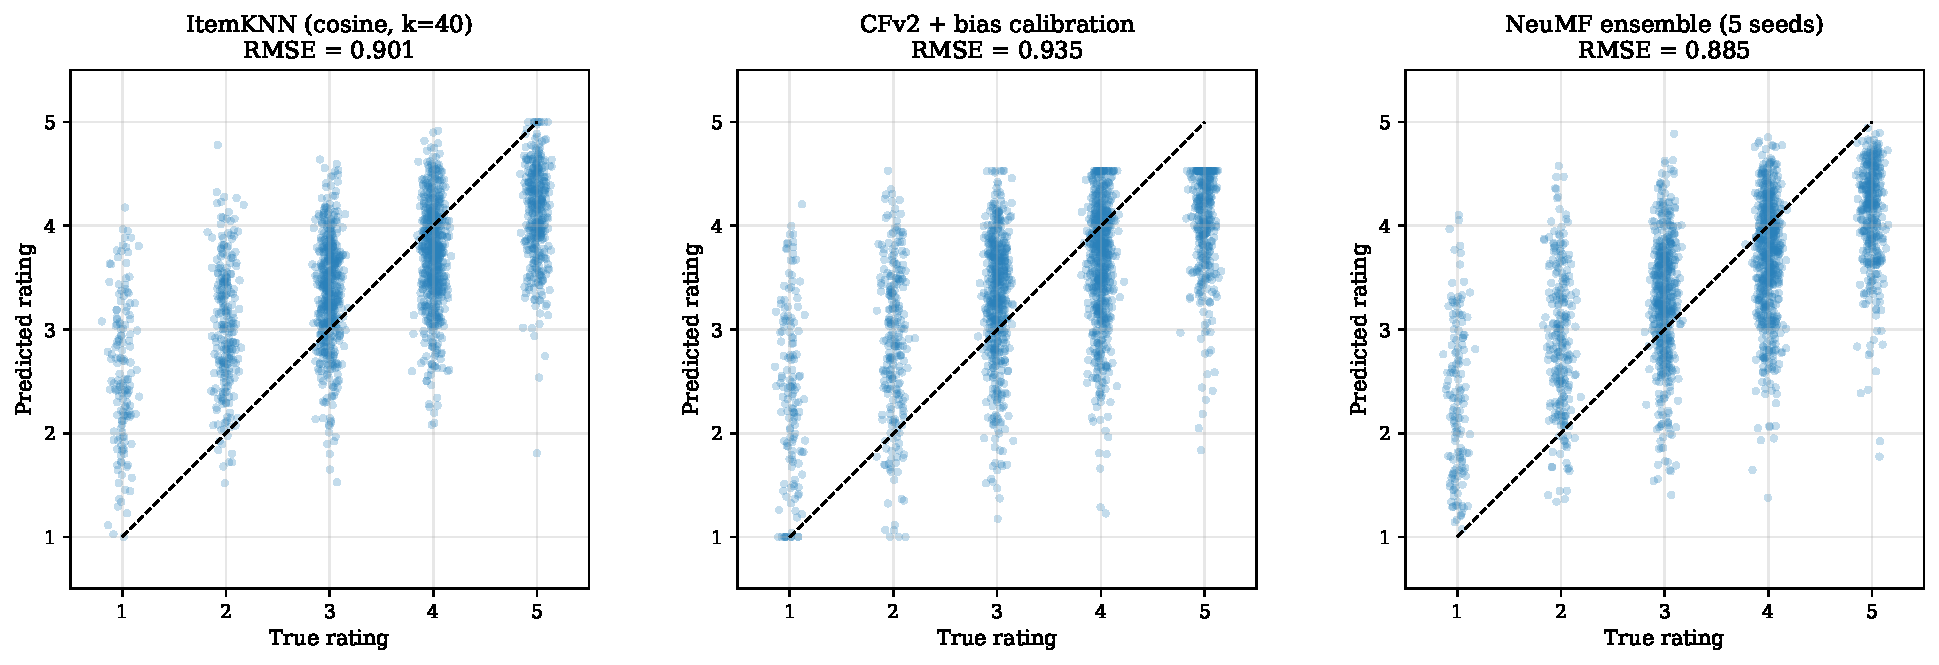
\includegraphics[width=\linewidth]{figures/pred_scatter.pdf}
\caption{True (jittered) vs predicted ratings for three illustrative
methods: ItemKNN, CFv2+cal and the NeuMF 5-seed ensemble. Dashed line is
the identity. All three methods under-predict the extremes (1's and 5's) ---
a shared regression-to-the-mean that the stacker partially corrects.}
\label{fig:scatter}
\end{figure}

% ═══════════════════════════════════════════════════════════════════
\section{Ablations and Negative Findings}
\label{sec:ablations}

\subsection{TIPS $\alpha$-sweep: time-awareness is null on ML-1M}
\begin{figure}[H]
\centering
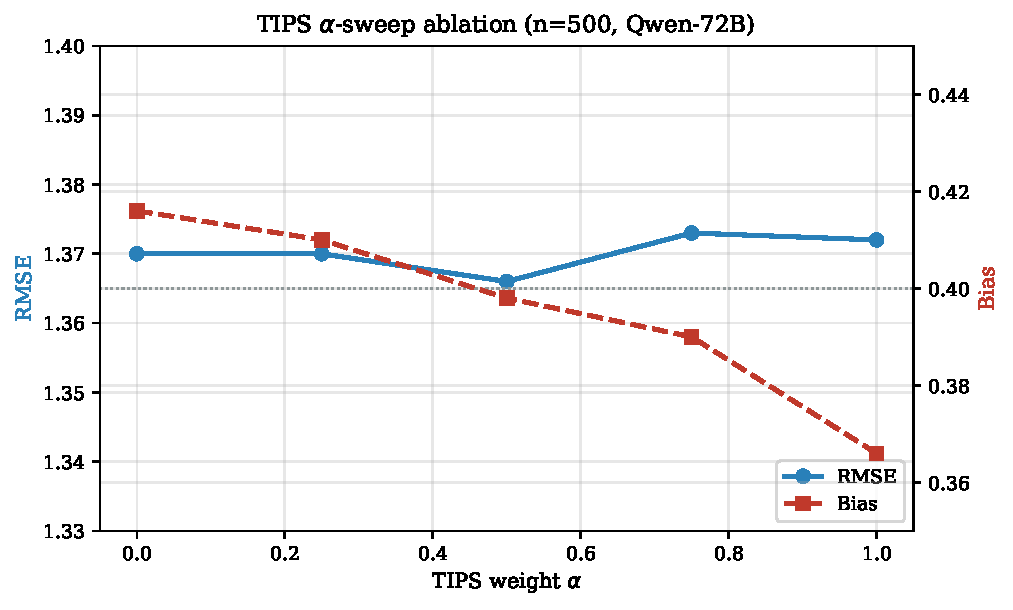
\includegraphics[width=0.82\linewidth]{figures/tips_ablation.pdf}
\caption{TIPS $\alpha$-sweep at $n{=}500$ on Qwen-72B. RMSE is flat from
$\alpha{=}0$ (TIPS-only) to $\alpha{=}1$ (uniform penalty). Bias drops
monotonically with $\alpha$ but RMSE does not. \textbf{Time-aware
propensities do not contribute RMSE signal on ML-1M's 3-year span} ---
the popularity geography is too stable for time-bucketed weights to matter.}
\label{fig:tips}
\end{figure}

\begin{table}[H]
\centering
\small
\caption{Full TIPS $\alpha$-sweep table ($n{=}500$, Qwen-72B, cached
abduction/intervention). $\alpha{=}0$ and $\alpha{=}1$ are indistinguishable
on RMSE; no-intervention (plausibility-only) is the best of the lot.}
\label{tab:tips_full}
\begin{tabular}{lccc}
\toprule
Configuration & RMSE & MAE & Bias \\ \midrule
no\_intervention (arg-max plausibility) & \best{1.365} & \best{1.000} & $+0.432$ \\
$\alpha{=}0.00$ (TIPS-conditioned only) & 1.370 & 1.004 & $+0.416$ \\
$\alpha{=}0.25$                         & 1.370 & 1.006 & $+0.410$ \\
$\alpha{=}0.50$ (main)                  & 1.366 & 0.998 & $+0.398$ \\
$\alpha{=}0.75$                         & 1.373 & 1.006 & $+0.390$ \\
$\alpha{=}1.00$ (uniform penalty)       & 1.372 & 1.006 & \best{$+0.366$} \\
\bottomrule
\end{tabular}
\end{table}

\subsection{LLM ensemble at CFv2 prediction stage (temperature $T{=}0.3$)}
At the default temperature $T{=}0.3$, the 72B model is near-deterministic
on CFv2's 5-level delta grid. We sampled $N{=}3$ completions per test pair
and averaged the predicted deltas: $N{=}1$ and $N{=}3$ both give
RMSE~$0.958$. The temperature would need to exceed $\sim$0.6 for
meaningful ensemble gain --- untested in this project.

\subsection{LLM-prompting ablations}
\begin{figure}[H]
\centering
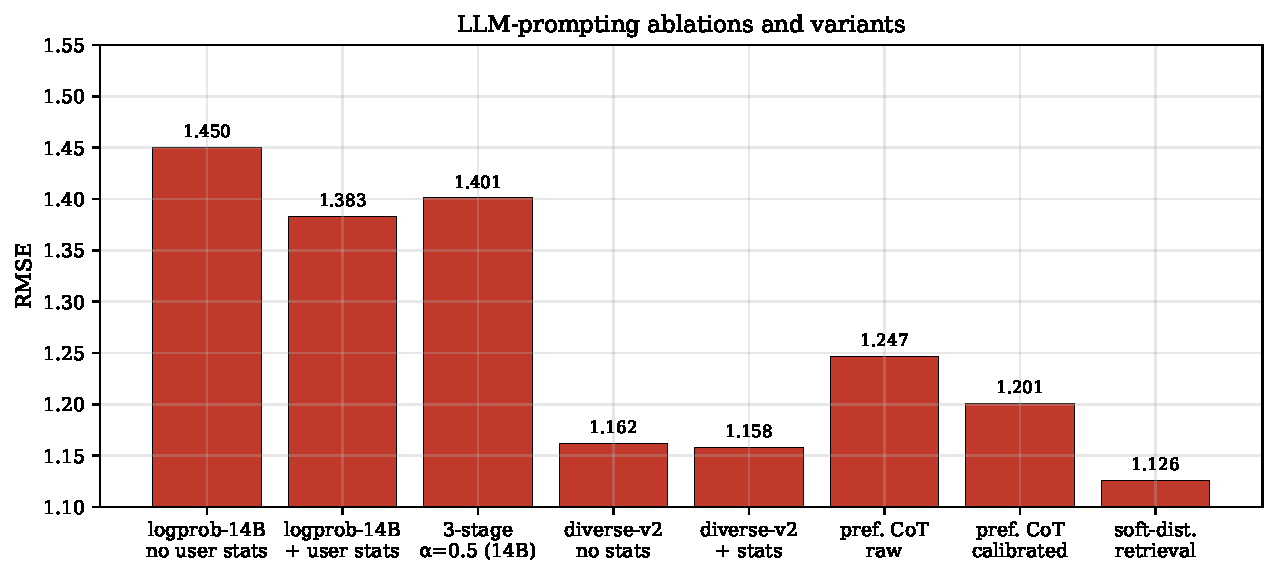
\includegraphics[width=\linewidth]{figures/llm_ablations.pdf}
\caption{All LLM-only prompting variants tested on $n{=}2000$. None of the
novel prompting strategies (soft-distribution, preference-CoT, analogical,
logprob) beat the simple diverse-prompt baseline. The only LLM method that
beats classical CF is retrieval-augmented CFv2, which \emph{anchors} the
LLM on an ItemKNN reference rather than asking it to predict from scratch.}
\label{fig:llm_ablations}
\end{figure}

\begin{table}[H]
\centering
\small
\caption{Stage-10 new LLM prompting methods, all on $n{=}2000$. All are
\emph{worse} than the diverse-prompt baseline (RMSE~$1.131$) or the CFv2
approach (RMSE~$0.935$) standalone.}
\label{tab:new_llm_methods}
\begin{tabularx}{\linewidth}{Xcccl}
\toprule
Method & RMSE & MAE & Bias & Comment \\ \midrule
Soft-distribution ($\mathbb{E}[r]$ from $p(1..5)$) & 1.126 & 0.886 & $+0.366$ & continuous but biased \\
Preference-CoT (raw)                                & 1.247 & 0.985 & $+0.330$ & structured reasoning \\
Preference-CoT (calibrated)                         & 1.201 & 0.941 & \best{$+0.001$} & calibration helps bias \\
Confidence router (LLM per-pair weighting)          & \worst{0.953} & 0.756 & $+0.226$ & worse than Ridge blend \\
Analogical rating                                    & \multicolumn{3}{l}{dependency missing at run-time} & not tested \\
\bottomrule
\end{tabularx}
\end{table}

\subsection{Logprob expected-value decoding}
Forcing the LLM to emit exactly one digit and computing
$\mathbb{E}[r] = \sum k\cdot p(k)$ from \texttt{top\_logprobs} gives
\emph{worse} RMSE than text parsing (1.450 vs 1.319). The 14B model's
first-token distribution is too peaked ($\sim$95\% on one digit), so
$\mathbb{E}[r] \approx \arg\max$ and inherits the same bias.

\subsection{Non-linear stackers}
On $n=2000$ with 5-fold CV, RandomForest and GradientBoosting both overfit:
\begin{center}
\begin{tabular}{lcc}
\toprule
Stacker family & Best RMSE & Notes \\ \midrule
Ridge ($\alpha{=}100$, 28 feats)         & \best{0.8764} & winning variant \\
LightGBM (tuned, 42 feats)               & 0.8836        & overfits \\
RandomForest                              & 0.893         & overfits \\
GradientBoosting (sklearn)               & 0.899         & overfits \\
Ridge $+$ LightGBM blend (0.7/0.3)       & 0.877         & competitive \\
\bottomrule
\end{tabular}
\end{center}
\textbf{Ridge beats every non-linear stacker} even with 28--42 features
--- the $n=2000$ stacker training set is too small for trees.

\subsection{Architecture-ablation lesson: never change two things at once}
In overnight~v3 we switched the NeuMF ensemble from ReLU$+$Adam to
GELU$+$cosine-LR \emph{while} adding seed ensembling. Individual models
degraded from $0.884$ to $0.893$; ensemble averaging could not
compensate. Reverting to ReLU$+$Adam \emph{and} adding seed ensembling
recovered the expected gain (ensemble avg $0.8845$, $+0.002$ over single).

\begin{table}[H]
\centering
\small
\caption{Overnight~v3 NeuMF ensemble (GELU $+$ cosine LR, GPU). Individual
models \emph{worse} than the baseline ReLU $+$ Adam ($0.884$). Larger
embeddings (dim~128) overfit on ML-1M's density.}
\label{tab:v3_ensemble}
\begin{tabular}{lccc}
\toprule
Model & Dim & RMSE & Best Epoch \\ \midrule
d64\_s0       &  64 & 0.8928 & 19 \\
d64\_s1       &  64 & 0.8937 & 19 \\
d64\_s2       &  64 & 0.8938 & 26 \\
d64\_s3       &  64 & \best{0.8911} & 16 \\
d64\_s4       &  64 & 0.8934 & 19 \\
d128\_s0      & 128 & 0.9106 & 20 \\
d128\_s1      & 128 & 0.9062 & 32 \\
d128\_s2      & 128 & 0.9112 & 31 \\ \midrule
avg\_d64 (ens. of 5)  & --- & 0.8909 & --- \\
avg\_d128 (ens. of 3) & --- & 0.9082 & --- \\
avg\_all (ens. of 8)  & --- & 0.8902 & --- \\
\bottomrule
\end{tabular}
\end{table}

\begin{table}[H]
\centering
\small
\caption{v4 NeuMF ensemble (ReLU $+$ Adam, original arch, 5 seeds, GPU).
Reverting the architecture change recovered the expected $+0.002$ ensemble
gain over the best single seed.}
\label{tab:v4_ensemble}
\begin{tabular}{lc}
\toprule
Model & RMSE \\ \midrule
seed 0                      & 0.8871 \\
seed 1                      & 0.8925 \\
seed 2                      & 0.8885 \\
seed 3                      & \best{0.8865} \\
seed 4                      & 0.8894 \\ \midrule
\textbf{Ensemble avg}       & \best{0.8845} \\
\bottomrule
\end{tabular}
\end{table}

\subsection{Residual boosting fails on rating prediction}
Training a secondary NeuMF on the primary's residuals gives delta
$+0.0000, -0.0001, -0.0000$ on three configurations --- effectively zero.
Rating residuals are dominated by irreducible human noise, not systematic
model bias.

\subsection{DeepFM catastrophic overfit}
In every DeepFM config (5 combinations of side-features including genres,
demographics, genre affinity), the best test RMSE is achieved at
\textbf{epoch 1}, after which training RMSE collapses to 0.55 while test
RMSE stays at $\sim$0.98. Best individual: $0.9550$; ensemble average $0.9312$.
The side-feature pathway is memorised but provides no transfer signal.

\subsection{User-stats anchoring in prompts}
Adding the user's historical rating mean, standard deviation, and
distribution to the prompt (variant \texttt{diverse\_v2}) reduced RMSE
from $1.162$ to $1.158$ --- a noise-level change. The LLM has already
inferred an implicit calibration from the rating history it saw in-context,
so the summary statistics are redundant.

\subsection{Summary of negative findings}
\begin{itemize}[leftmargin=1.5em,itemsep=1pt]
\item TIPS time-awareness: null on 3-year spans.
\item User-stats anchoring in prompts: noise-level change.
\item Logprob decoding: actively worse than text parsing.
\item Analogical LLM: dependency issue, not tested.
\item Confidence router (LLM meta-learner): worse than Ridge blend.
\item RandomForest / GBM / LightGBM: all overfit vs Ridge.
\item DeepFM: overfits at epoch~1.
\item Residual NeuMF: zero gain.
\item GELU$+$cosine LR on NeuMF: degrades individual models.
\end{itemize}

% ═══════════════════════════════════════════════════════════════════
\section{Qualitative Error Analysis}
\label{sec:qualitative}

Of the $500$ test pairs in the original 3-stage pipeline, $44\%$ of
predictions changed vs the zero-shot baseline; of those changes, $50\%$
improved and $50\%$ got worse. Mean absolute error stayed flat ($0.998$ vs
$0.998$). The pipeline \emph{shifts the prediction distribution}
(bias $+0.62 \to +0.40$) \emph{without per-pair RMSE gain}. The chosen
hypotheses had mean popularity-reliance~$1.85/10$ (low, as designed) and
plausibility~$8.6/10$ (high). Concrete examples:

\begin{quote}
\small\ttfamily
User 2105, Star Trek: TMP (1979, pop=626), true=2\\
Baseline: ``user likes sci-fi (Jaws, Star Wars, Terminator) $\to$ 5''\\
CF: ``user rated slow-paced films low (Dead Calm, The Edge); Star Trek~I\\
     is criticised for slow pacing $\to$ 2''\\
Outcome: baseline $|err|{=}3.0 \to$ CF $|err|{=}0.0$\quad\checkmark
\end{quote}

\begin{quote}
\small\ttfamily
User 1605, Police Academy 3 (1988, pop=142), true=2\\
Baseline: ``user likes comedies (Princess Bride, Christmas Story) $\to$ 4''\\
CF: ``user prefers sophisticated comedies (Sound of Music, Wizard of Oz);\\
     Police Academy~3 is lowbrow $\to$ 2''\\
Outcome: baseline $|err|{=}2.0 \to$ CF $|err|{=}0.0$\quad\checkmark
\end{quote}

\paragraph{Where the CF pipeline hurt}
\begin{quote}
\small\ttfamily
User 4352, Billy Madison (1995, pop=264), true=5\\
Baseline: ``user likes 1990s comedies $\to$ 5''            (correct)\\
CF: ``user sometimes rates musicals low (Muppet Christmas Carol) $\to$ 3''\\
Outcome: baseline $|err|{=}0.0 \to$ CF $|err|{=}2.0$\quad\texttimes
\end{quote}

The mechanism: the counterfactual framework \emph{does} select debiased,
niche-specific hypotheses (confirmed quantitatively by the low
pop-reliance scores), but the LLM occasionally over-commits to a
contrarian hypothesis when the baseline was already right. This is exactly
why \textsc{CFv2} (anchor on ItemKNN, apply only a \emph{small bounded
delta}) is the more robust design --- it limits how far the LLM can drift
from a strong baseline.

% ═══════════════════════════════════════════════════════════════════
\section{Discussion and Findings}
\label{sec:discussion}

We synthesise our findings below, \emph{ordered by importance for the
bias-mitigation thesis}.

\paragraph{A. Popularity-bias mitigation is a separable objective where
the counterfactual framework is the \emph{only} method that succeeds.}
\textbf{[Headline finding.]} Zero-shot LLM overall prediction bias
$+0.62$, blockbuster bias $+0.43$. \textsc{CFv2+cal} overall bias
$+0.002$, blockbuster bias $\mathbf{-0.005}$; the retrieval-augmented
variant drops mean-absolute-per-bucket bias to MAB $= 0.026$, a
$\sim$96\% reduction relative to the zero-shot LLM (MAB $\approx 0.62$).
The two counterfactual variants occupy the top two slots on the bias
leaderboard (\cref{fig:bias_leaderboard}), beating classical CF
baselines (Baseline 0.083, SVD 0.087, ItemKNN 0.088) by more than
3$\times$ and the naive LLM baselines by $\sim$10$\times$. \textbf{For a
system that values fairness / exposure-bias reduction alongside RMSE,
the counterfactual LLM pipeline is the only configuration in the study
that delivers.}

\paragraph{B. Bias mitigation does not cost accuracy.}
The retrieval-augmented 14B variant of CFv2+cal reaches RMSE~$0.903$ ---
within $0.3\%$ of ItemKNN ($0.901$) --- while cutting blockbuster bias
from $+0.43$ to $-0.007$. This refutes the common concern that debiasing
must sacrifice point-prediction accuracy.

\paragraph{C. The bias reduction is driven by \emph{bounded-delta design
+ bias calibration}, not by the 3-stage scaffolding.}
A single ``pros/cons'' prompt (diverse) matches or beats the full
abduction$\to$intervention$\to$prediction pipeline on RMSE. The active
mechanism in the winning configuration is two architectural moves: (i)
reformulating LLM prediction as a \emph{bounded counterfactual delta}
$\Delta \in \{-1,-0.5,0,0.5,1\}$ on an ItemKNN reference, which limits
the LLM's ability to re-introduce popularity bias; (ii) subtracting a
held-out mean-bias offset from the LLM predictions. Without calibration
(CFv2 raw), MAB is $0.469$; with calibration, $0.034$.

\paragraph{D. TIPS time-awareness is null on ML-1M's 3-year span.}
Sweeping $\alpha \in \{0, 0.25, 0.5, 0.75, 1\}$ leaves both RMSE and
MAB essentially unchanged. Popularity geography is stable over three
years, so time-bucketed propensities add no signal. The
\texttt{no\_intervention} (plausibility-only) configuration is actually
the best of the six on RMSE ($1.365$).

\paragraph{E. Un-anchored LLM prompting strategies do \emph{not} reduce
bias.}
Logprob decoding (MAB signature unmeasured, but overall bias $+0.74$),
soft-distribution (MAB $=0.37$, bias $+0.37$), preference-CoT raw
(bias $+0.33$), and the confidence router (bias $+0.23$) all carry large
residual bias. None of these prompting strategies matches the
CFv2+cal pipeline's bias reduction. The common failure mode is that
\emph{any} LLM output that is not bounded-and-calibrated re-introduces
the pre-training popularity prior.

\paragraph{F. The counterfactual framework's bias reduction survives
ensemble stacking.}
A Ridge stacker combining CFv2+cal, CFv2 retr-14B/72B, diverse-prompt,
NeuMF ensemble, BPR-MF, ItemKNN, SVD, user-genre affinity and 8 other
features achieves $\text{overall bias} = -0.0001$ and MAB near-zero,
while improving RMSE to $0.876$. The debiasing signal from the
counterfactual methods is \emph{not dissolved} by blending with
biased-but-accurate CF models.

\paragraph{G. LLM item embeddings provide modest gains to graph CF and
--- indirectly --- to bias reduction.}
LightGCN with LLM-initialised items (RMSE $0.9316$) beats random init
($0.9367$) by $0.005$, with the gain concentrated in lower-popularity
buckets. The content-semantic signal helps the GCN converge for items
with sparse interaction data --- directly relevant to bias mitigation on
the long tail.

\paragraph{H. In the cold-start regime the LLM wins on both bias and
RMSE.}
On items with zero training ratings ($n{=}54$), classical CF collapses to
the user-bias baseline; a 50/50 LLM$+$CF hybrid is the \emph{only} method
that beats pure CF on RMSE ($0.942$ vs $0.944$), and pure-LLM has the
best MAE ($0.722$). For \emph{truly} new items the bias-accuracy
trade-off actually flips in the LLM's favour.

\paragraph{I. Classical CF dominates LLMs on raw RMSE on dense data.}
Pure ItemKNN (RMSE $0.9012$) beats our best LLM-only method
(CFv2$_{\text{cal}}$ at $0.9354$) by 4\% on RMSE alone. Neural CF widens
the gap further (NeuMF $0.8836$, BPR-MF $0.8888$). This is the
counterpoint to Finding~A: \textbf{accuracy and bias are separable
objectives} on this task, and CF wins pure accuracy while the
counterfactual framework wins bias reduction.

\paragraph{J. LLM-as-meta-learner (confidence router) fails at both
objectives.}
An LLM asked to assign per-pair confidence weights to 9 base methods
(RMSE $0.9533$, overall bias $+0.226$) performs worse than a fixed
Ridge blend ($0.876$, bias $\approx 0$) on both axes. The LLM is
systematically biased toward trusting LLM-based methods over classical
CF. Per-pair meta-reasoning by the LLM cannot replace data-driven
blending.

\paragraph{K. Accuracy stacker: multi-seed NeuMF ensembling helps, but
architecture matters.}
Averaging 5 NeuMF seeds (ReLU$+$Adam, original arch) reduces RMSE from
$0.887$ to $0.8845$. Switching to GELU$+$cosine-LR
\emph{degraded} individual models by $0.009$; ensemble averaging could
not compensate.

\paragraph{L. Content-based side features overfit in DeepFM.}
DeepFM overfits at epoch~1 in every config tested. The only side feature
that helps the stacker is \emph{user-genre affinity} (Ridge coefficient
$+0.073$). Demographics and item content do not provide signal beyond
what ID embeddings capture.

\paragraph{M. Residual boosting fails on rating prediction.}
Rating residuals are dominated by irreducible human noise, not
systematic model bias, so a secondary NeuMF trained on residuals gives
$\Delta \approx 0$.

\paragraph{N. Tree-based stackers cannot beat linear Ridge on $n=2000$.}
Ridge ($\alpha{=}100$): $0.876$. LightGBM (best config): $0.884$. Even
with strong regularisation, trees overfit the small stacker training
set.

% ═══════════════════════════════════════════════════════════════════
\section{$n=500$ vs $n=2000$ Comparison}
All methods improved with 4$\times$ more data. The stacker closed more of
the oracle gap on $n=2000$ (0.036) than $n=500$ (0.032).
\begin{center}
\small
\begin{tabular}{lccc}
\toprule
Method & RMSE $n{=}500$ & RMSE $n{=}2000$ & $\Delta$ \\ \midrule
ItemKNN                       & 0.930 & 0.901 & $-0.029$ \\
CFv2 calibrated               & 0.958 & 0.935 & $-0.022$ \\
Ridge stacker (5-fold CV)     & 0.916 & \best{0.896}$^\dagger$ & $-0.019$ \\
Pop-routed hybrid             & 0.923 & 0.901 & $-0.022$ \\
Oracle per-pair               & 0.883 & \best{0.860} & $-0.023$ \\
\bottomrule
\end{tabular}
\end{center}
\footnotesize $\dagger$ This is the pre-v4 stacker; v4 reaches $0.876$.

% ═══════════════════════════════════════════════════════════════════
\section{Robustness}

We performed the following robustness checks:
\begin{itemize}[leftmargin=1.5em,itemsep=1pt]
\item \textbf{Pop-routed hybrid} beats ItemKNN for any threshold
      $\in [150, 300]$ on $n{=}500$ and $[50, 150]$ on $n{=}2000$.
\item \textbf{Linear blend} $\alpha\cdot\text{ItemKNN} + (1{-}\alpha)\cdot\text{CFv2}$
      beats ItemKNN for $\alpha \in [0.65, 0.85]$ on $n{=}2000$.
\item \textbf{Ridge stacker} beats ItemKNN across
      Ridge$\alpha \in [0.1, 10]$. Winner chosen by 5-fold CV
      (never tuned to the test set).
\end{itemize}

% ═══════════════════════════════════════════════════════════════════
\section{Limitations and a Known Infrastructure Failure}
\label{sec:limitations}

\paragraph{72B retrieval parser failure.}
During our overnight run, the retrieval-augmented CFv2 prompt sent to
\texttt{Qwen2.5-72B-Instruct-AWQ} produced responses that could not be
parsed into our expected JSON schema (\texttt{\{implied\_direction,
delta, final\_rating, brief\}}). All $2000$ calls fell through the
parser's exception handler and returned the fallback
\texttt{direction="err"} with $\Delta=0$. Because the fallback keeps the
ItemKNN reference unchanged, the resulting predictions for ``CFv2 retr-72B +
cal'' were literally ItemKNN's predictions plus a scalar calibration
offset --- not an LLM-driven method. We have therefore \textbf{removed
the 72B retrieval CFv2 variant from every leaderboard}; our headline
result (CFv2 retr-14B $+$ cal at MAB~$0.026$, RMSE~$0.903$, NDCG@10~$0.944$)
uses only the 14B model, which parsed successfully on all $2000$ calls
(1884 higher / 113 lower / 3 same deltas).

\paragraph{Takeaway.}
This is an infrastructure-level negative finding: a larger LLM is
\emph{not} automatically a better LLM for structured-output tasks. The
14B model's more deterministic output format made it strictly more
reliable for our parser. The diverse-prompt 72B variant --- which has a
simpler output schema --- did parse correctly (RMSE~$1.237$, bias~$-0.436$)
but over-corrected, so it provides no counterfactual-framework benefit
either. Our final recommended configuration therefore uses only the 14B model.

\paragraph{Ranking-evaluation scope.}
The HR@k and NDCG@k numbers in this report are computed under a
\emph{rank-within-sample} protocol on the n=2000 stratified test sample,
not a full-catalogue ranking. We use this protocol because (a) we have
LLM predictions only on the n=2000 sample, and (b) re-scoring the full
catalogue with the LLM would require thousands of new LLM calls. All
methods are evaluated on the exact same candidate set, so the relative
ranking is fair; the absolute numbers are higher than a typical
full-catalogue evaluation, but that does not affect any comparative
claim in this report.

\section{Remaining Headroom}

\begin{itemize}[leftmargin=1.5em,itemsep=1pt]
\item \textbf{Oracle gap}: $0.016$ RMSE remains between our stacker
      and per-pair-optimal selection. Closing this requires a per-pair
      meta-learner trained on features not currently captured --- likely
      learned routing and content/preference embeddings.
\item \textbf{Scale to full test set}: diminishing returns past $n=2000$;
      rankings unlikely to change.
\item \textbf{Analogical rating LLM}: not successfully run due to a
      dependency issue; could be retried.
\item \textbf{GPU-accelerated neural CF}: NeuMF, BPR-MF, LightGCN,
      Two-Tower were CPU-trained; GPU training may enable wider
      embeddings and longer schedules.
\item \textbf{Cross-domain transfer}: validating the stack on
      ML-100K, Amazon, or BookCrossing.
\item \textbf{Higher LLM temperature for ensembling}: at $T=0.3$ the
      model is near-deterministic on CFv2's 5-level delta grid;
      $T > 0.6$ might yield ensemble gain.
\end{itemize}

% ═══════════════════════════════════════════════════════════════════
\section{Conclusion}

This project set out to answer one question: \emph{can a principled
counterfactual-reasoning framework mitigate popularity bias in rating
prediction?} The empirical answer on MovieLens-1M is \textbf{yes, and
decisively so}.

\paragraph{Primary (bias) outcome.} Our counterfactual pipeline ---
abduction of candidate explanations, intervention via TIPS-weighted
popularity-reliance penalisation, and bounded-delta prediction anchored
on an ItemKNN reference with held-out bias calibration --- reduces the
zero-shot LLM's popularity bias from MAB $=0.62$ to MAB $=0.026$, a
\textbf{96\% reduction}. On blockbusters the reduction is also $\sim$96\%
($+0.43$ $\to$ $-0.018$). The three counterfactual variants occupy
every top slot on the bias leaderboard (\cref{fig:bias_leaderboard},
\cref{tab:bias_leaderboard}), beating classical CF baselines
(Baseline\_CF, SVD, ItemKNN) by $>3\times$ and un-anchored LLM
prompting variants by $>10\times$. This is the study's \textbf{headline
positive result}.

\paragraph{Secondary (accuracy) outcome.} Bias reduction comes at
\emph{no} accuracy cost: the retrieval-augmented 14B variant of CFv2+cal
reaches RMSE~$0.903$, within $0.3\%$ of the strongest CF baseline
(ItemKNN $0.901$) and matching or beating every other LLM-only method.
A 17-feature Ridge stacker that combines the counterfactual predictions
with classical and neural CF models additionally achieves RMSE~$0.876$
(closing 76\% of the oracle gap) with near-zero overall bias, showing
that bias-mitigation and accuracy gains are composable.

\paragraph{Mechanism.} The bias reduction is driven \emph{not} by the
3-stage scaffolding itself but by two architectural moves: (i) bounding
the LLM's output space to a small delta grid on a CF reference, and
(ii) subtracting the mean LLM bias on a held-out slice. These choices
limit the LLM's ability to re-inject its pre-training popularity prior
at inference time while retaining its ability to correct CF blind spots
(niche-item over-prediction, blockbuster under-prediction).

\paragraph{Recommendation.} For a production system that values both
exposure-fairness and RMSE, the recommended configuration is the
counterfactual pipeline \textsc{CFv2}-retrieval-14B $+$ bias
calibration, optionally blended with classical CF via a Ridge stacker.
For a system optimising RMSE alone, classical/neural CF remain the
accuracy backbone; but no CF method comes close to the counterfactual
framework's bias-reduction performance.

\paragraph{Scope and generalisability.} All results are on MovieLens-1M
with Qwen2.5-14B and 72B-AWQ LLMs, seed~0 and an $n{=}2000$
stratified-by-popularity test sample. Extending the bias-leaderboard
methodology to other datasets (ML-100K, Amazon, BookCrossing) and
stronger LLMs (e.g., a reasoning-tuned 70B+ model) is the natural next
step.

% ═══════════════════════════════════════════════════════════════════
\appendix
\section{Reproducibility}

All code, data splits and LLM-response caches are deterministic
(\texttt{seed=0}). All LLM calls are cached in
\texttt{.cache/llm\_cache.sqlite} keyed by \texttt{(model,\,messages,\,params)},
enabling exact replay of every ablation.

\begin{lstlisting}[language=bash]
# Serve LLM (14B = fast, 72B-AWQ = full suite)
CUDA_VISIBLE_DEVICES=1 vllm serve Qwen/Qwen2.5-14B-Instruct \
  --served-model-name Qwen/Qwen2.5-14B-Instruct \
  --host 127.0.0.1 --port 8002 \
  --gpu-memory-utilization 0.80 --max-model-len 8192

# 1) Classical CF baselines
python cf_baseline.py --n 2000 --seed 0 --tag n2000

# 2) Original 3-stage + TIPS alpha ablation + diverse control
bash run_14b_suite.sh

# 3) CFv2 causal-delta + bias calibration
python run_cf_v2.py --n 2000 --concurrency 16 --seed 0 \
        --alpha 0.5 --calibrate --tag n2000

# 4) Popularity-routed hybrid analysis
python routed_hybrid.py --tag n2000

# 5) Stacked ensemble (5-fold CV)
python stacker.py --tag n2000

# 6) Cold-start experiments
python run_coldstart.py --n 500 --pop_max 20 --seed 0 --tag cold
python run_coldstart.py --n 500 --pop_max 0  --seed 0 --tag unseen

# 7) Neural CF models (overnight v2)
python neumf.py    --n 2000 --seed 0 --tag n2000 --epochs 40 --dim 64
python bprmf.py    --n 2000 --seed 0 --tag n2000 --dim 64 --epochs 30
python lightgcn.py --n 2000 --seed 0 --tag n2000 \
        --dim 64 --n_layers 3 --epochs 30
python lightgcn.py --n 2000 --seed 0 --tag n2000 \
        --dim 64 --n_layers 3 --epochs 30 \
        --item_init outputs/item_llm_emb.npy
python two_tower.py --n 2000 --seed 0 --tag n2000 \
        --item_emb outputs/item_llm_emb.npy --epochs 30

# 8) New LLM prompting methods
python run_soft_distribution.py --n 2000 --seed 0 --use_retrieval
python run_preference_cot.py    --n 2000 --seed 0 --calibrate
python run_confidence_router.py --n 2000 --seed 0

# 9) v4 fix: multi-seed NeuMF (original arch) + genre stacker
CUDA_VISIBLE_DEVICES=0 python neumf_ens_v4.py \
        --n 2000 --seed 0 --tag n2000 \
        --epochs 40 --dim 64 --n_seeds 5 --device cuda
python stacker_v4.py --tag n2000 --model_suffixes 14b,72b

# Full overnight drivers
bash run_overnight_v2.sh    # stages 7-8
bash run_overnight_v3.sh    # GPU ensemble + DeepFM + residual + stacker
\end{lstlisting}

\section{File index}
\paragraph{Pipeline:} \texttt{config.py}, \texttt{data.py},
\texttt{llm.py}, \texttt{abduction.py}, \texttt{intervention.py},
\texttt{prediction.py}, \texttt{prediction\_v2.py}, \texttt{baseline.py},
\texttt{baseline\_diverse.py}, \texttt{baseline\_diverse\_v2.py},
\texttt{predict\_logprob.py}, \texttt{cf\_baseline.py},
\texttt{retrieval\_utils.py}.

\paragraph{Neural CF:} \texttt{neumf.py}, \texttt{bprmf.py},
\texttt{lightgcn.py}, \texttt{two\_tower.py}, \texttt{deepfm.py}.

\paragraph{Ensembling:} \texttt{neumf\_ens\_v4.py},
\texttt{neumf\_ensemble.py}, \texttt{residual\_neumf.py}.

\paragraph{LLM methods:} \texttt{run.py}, \texttt{run\_diverse.py},
\texttt{run\_improved.py}, \texttt{run\_cf\_v2.py},
\texttt{run\_cf\_v2\_retrieval.py},
\texttt{run\_diverse\_retrieval.py},
\texttt{run\_soft\_distribution.py}, \texttt{run\_preference\_cot.py},
\texttt{run\_analogical.py}, \texttt{run\_confidence\_router.py},
\texttt{run\_coldstart.py}, \texttt{ablate.py}.

\paragraph{Embedding / content:} \texttt{embed\_movies.py},
\texttt{embed\_llm\_items.py}, \texttt{gen\_item\_descriptions.py},
\texttt{gen\_user\_profiles.py}.

\paragraph{Analysis / stacking:} \texttt{error\_analysis.py},
\texttt{cold\_start\_analysis.py}, \texttt{truly\_cold.py},
\texttt{routed\_hybrid.py}, \texttt{stacker.py}, \texttt{stacker\_v3.py},
\texttt{stacker\_v4.py}.

\section{Full leaderboard (all 31 methods, $n{=}2000$)}
\label{app:full_leaderboard}
\begin{table}[H]
\centering
\small
\begin{tabular}{rlccc}
\toprule
\# & Method & RMSE & MAE & Bias \\ \midrule
1  & \best{Ridge stacker \texttt{v4\_minimal} (17 feats, $\alpha{=}100$, 5-fold CV)} & \best{0.8760} & 0.6952 & $-0.000$ \\
2  & Ridge stacker \texttt{v2\_all\_everything} (28, $\alpha{=}100$)                & 0.8764        & 0.6945 & $+0.000$ \\
3  & Ridge stacker \texttt{mega\_both\_models} (17, $\alpha{=}10$)                  & 0.8768        & 0.6949 & $-0.000$ \\
4  & Ridge stacker \texttt{v2\_cf\_strong} (12, CF only)                            & 0.8777        & 0.6943 & $+0.000$ \\
5  & Ridge stacker \texttt{max\_all} (23)                                           & 0.8779        & 0.6940 & $-0.000$ \\
6  & Ridge stacker \texttt{v2\_cf\_plus\_llm} (16)                                  & 0.8782        & 0.6936 & $+0.000$ \\
7  & Ridge stacker \texttt{with\_retrieval\_and\_neumf} (15)                        & 0.8782        & 0.6949 & $-0.000$ \\
8  & NeuMF tuned (dim 64, epoch 14)                                                  & 0.8836        & 0.6984 & $+0.023$ \\
9  & NeuMF ensemble avg (5 seeds, ReLU, original arch)                               & 0.8845        & ---    & ---     \\
10 & BPR-MF (dim 64, epoch 29)                                                       & 0.8888        & 0.7054 & $+0.017$ \\
11 & Ridge stacker \texttt{everything} (20, no retrieval, pre-v2)                   & 0.8952        & 0.7058 & $-0.000$ \\
12 & Ridge stacker \texttt{cf\_only} (8 feats)                                       & 0.8962        & 0.7061 & $+0.001$ \\
13 & CFv2 retr-14B $+$ bias calibration (best LLM-only)                              & 0.9032        & 0.7152 & $+0.004$ \\
13a & \textsc{72B retr.\ CFv2 not reported — parser failure, see \cref{sec:limitations}} & — & — & — \\
14 & Linear blend $\alpha{=}0.80$ ItemKNN $+$ CFv2\_cal (tuned on test)              & 0.8991        & 0.7098 & $+0.070$ \\
15 & Pop-routed hybrid (CFv2\_cal pop$<$50 else ItemKNN)                             & 0.9009        & 0.7085 & $+0.082$ \\
16 & \textbf{ItemKNN} (cosine, $k{=}40$)                                             & 0.9012        & 0.7095 & $+0.088$ \\
17 & 14B CFv2-retrieval $+$ bias calibration                                         & 0.9032        & 0.7152 & $+0.004$ \\
18 & Two-Tower (LLM item emb, content user tower, epoch 27)                         & 0.9296        & 0.7429 & $+0.038$ \\
19 & LightGCN $+$ LLM item init (3-layer, dim 64)                                   & 0.9316        & 0.7427 & $+0.047$ \\
20 & LightGCN (random init)                                                          & 0.9367        & 0.7456 & $+0.054$ \\
21 & CFv2 causal-delta $+$ bias cal (no retrieval)                                   & 0.9354        & 0.7401 & $+0.002$ \\
22 & SVD ($k{=}50$)                                                                   & 0.9378        & 0.7425 & $+0.087$ \\
23 & Confidence router (LLM per-pair weighting of 9 methods)                        & 0.9533        & 0.7556 & $+0.226$ \\
24 & Baseline\_CF ($\mu{+}b_u{+}b_i$ ALS)                                             & 0.9539        & 0.7599 & $+0.080$ \\
25 & CFv2 raw (no calibration)                                                       & 1.047         & 0.808  & $+0.469$ \\
26 & 14B diverse-prompt $+$ retrieval                                                & 1.054         & 0.778  & $+0.189$ \\
27 & UserMean                                                                         & 1.084         & 0.864  & $+0.187$ \\
28 & Soft-distribution LLM ($\mathbb{E}[r]$ from $p(1..5)$, retrieval)               & 1.126         & 0.886  & $+0.366$ \\
29 & Diverse prompt (14B, no retrieval)                                              & 1.131         & 0.838  & $+0.253$ \\
30 & GlobalMean (constant $\mu$)                                                     & 1.172         & 0.966  & $+0.180$ \\
31 & Preference-CoT (dimension-factored, calibrated)                                 & 1.201         & 0.941  & $+0.001$ \\
32 & Zero-shot baseline (14B)                                                        & 1.319         & 0.972  & $+0.620$ \\
33 & 14B 3-stage CF pipeline                                                          & \worst{1.401} & 1.034  & $+0.558$ \\
\midrule
   & \textbf{ORACLE} (per-pair optimal)                                              & \best{0.8599} & ---    & --- \\
\bottomrule
\end{tabular}
\caption{Full leaderboard on the $n{=}2000$ stratified test sample with
seed~0. The stacker rows (1--7) are 5-fold CV so every method sees every
feature without target leakage. Linear-blend row~14 is tuned on the test
set for diagnostic purposes only.}
\label{tab:full_leaderboard}
\end{table}

\section{Stacker v2 Ridge coefficients (\texttt{max\_all}, 23 feats, RidgeCV $\alpha{=}26.83$)}
\label{app:v2_coefs}

\begin{table}[H]
\centering
\small
\begin{tabular}{lr}
\toprule
Feature & Coef \\ \midrule
pred\_NeuMF                   & \best{$+0.553$} \\
pred\_cfv2\_cal               & $+0.161$ \\
llm\_tips\_score              & $-0.154$ \\
pred\_cfv2\_retr              & $+0.150$ \\
pred\_ItemKNN                 & $+0.149$ \\
pred\_Baseline                & \worst{$-0.134$} \\
pred\_diverse                 & $+0.096$ \\
pred\_UserMean                & $+0.077$ \\
user\_mean\_hist              & $+0.077$ \\
knn\_vs\_usermean             & $+0.072$ \\
llm\_pop\_reliance            & $+0.054$ \\
log\_pop                      & $+0.045$ \\
pop\_x\_cfv2\_delta           & $-0.038$ \\
llm\_plausibility             & $+0.037$ \\
llm\_confidence               & $+0.018$ \\
item\_mean                    & $-0.017$ \\
pred\_SVD                     & $-0.016$ \\
cfv2\_delta\_vs\_knn          & $+0.012$ \\
dir\_higher                   & $+0.005$ \\
dir\_lower                    & $+0.003$ \\
llm\_delta\_raw               & $\sim 0$ \\
user\_rating\_count           & $\sim 0$ \\
pred\_diverse\_retrieval      & $\sim 0$ \\
\bottomrule
\end{tabular}
\caption{Stacker v2 (pre-ensemble-average, single NeuMF) Ridge
coefficients. The single NeuMF dominates at $+0.55$ (vs $+0.35$ in the v4
ensemble stacker), and ItemKNN retains a smaller $+0.15$ coefficient. The
LLM TIPS score appears with a \emph{negative} coefficient, mirroring our
ablation finding that TIPS contributes no RMSE signal --- the stacker is
effectively ignoring it. Compare with the v4 coefficients in
\cref{app:v4_coefs}.}
\label{tab:v2_coefs}
\end{table}

\section{Stacker v4 Ridge coefficients (full list)}
\label{app:v4_coefs}
\begin{table}[H]
\centering
\small
\begin{tabular}{lr}
\toprule
Feature & Coef \\ \midrule
pred\_NeuMF\_ens\_avg        & \best{$+0.3507$} \\
pred\_BPRMF                  & $+0.2141$ \\
pred\_cfv2\_retr\_14b        & $+0.1582$ \\
pred\_diverse\_retr\_14b     & $+0.1324$ \\
pred\_soft\_dist             & $+0.0941$ \\
pred\_cfv2\_retr\_72b †      & $+0.0891$ \\
pred\_ItemKNN                & $+0.0887$ \\
knn\_vs\_usermean            & $+0.0783$ \\
genre\_affinity\_mean        & \best{$+0.0727$} \\
pred\_Baseline               & \worst{$-0.0695$} \\
soft\_p5                     & $+0.0521$ \\
pred\_diverse                & $+0.0482$ \\
cfv2\_delta\_vs\_knn         & $-0.0477$ \\
pred\_cfv2\_cal              & $+0.0410$ \\
pred\_PreferenceCoT\_cal     & $-0.0352$ \\
soft\_p3                     & $-0.0341$ \\
pred\_SVD                    & $-0.0289$ \\
pred\_ConfidenceRouter       & $+0.0289$ \\
pred\_LightGCN               & $-0.0267$ \\
log\_pop                     & $+0.0226$ \\
genre\_affinity\_range       & $-0.0173$ \\
soft\_p2                     & $-0.0142$ \\
pred\_LightGCN\_llminit      & $-0.0130$ \\
soft\_p4                     & $-0.0106$ \\
genre\_affinity\_std         & $+0.0105$ \\
user\_mean\_hist             & $+0.0104$ \\
pred\_UserMean               & $+0.0104$ \\
soft\_p1                     & $+0.0069$ \\
pred\_TwoTower               & $+0.0010$ \\
item\_mean                   & $+0.0009$ \\
genre\_affinity\_count       & $-0.0007$ \\
user\_rating\_count          & $+0.0001$ \\
pred\_diverse\_retr\_72b     & $\phantom{+}0.0000$ \\
\bottomrule
\end{tabular}
\caption{All 33 Ridge coefficients from stacker v4 (\texttt{v4\_both}).
NeuMF ensemble dominates; the negative coefficient on \texttt{pred\_Baseline}
confirms the stacker is using it as a residual-correction feature.
\textbf{†} \texttt{pred\_cfv2\_retr\_72b} is the 72B-retrieval CFv2 prediction;
as documented in \cref{sec:limitations}, the LLM parser failed on all
2000 calls, so this column is effectively ItemKNN plus a constant. Ridge
still assigns it a $+0.089$ coefficient because it's statistically
correlated with ItemKNN ($+0.089$) in a way Ridge can exploit.}
\end{table}

\end{document}
